% Sumber LaTeX untuk buku ``Metode Aljabar'' dalam bahasa Tionghoa
% Hak cipta 2018 Wen-Wei Li.
% Izin diberikan untuk menyalin, mendistribusikan, dan/atau mengubah
% dokumen ini berdasarkan ketentuan Creative Commons
% Atribusi 4.0 Internasional (CC BY 4.0)
% http://creativecommons.org/licenses/by/4.0/

% Untuk disertakan
\chapter{Kategori Monoidal}\label{sec:monoidal-cat}
Kategori monoidal semula disebut ``kategori dengan perkalian''. Kategori ini dilengkapi struktur berupa operasi $\otimes$ yang menyerupai perkalian dan objek satuan $\munit$, beserta kendala-kendala seperti sifat asosiatif dan sifat unsur satuan hingga isomorfisme natural. Kategori monoidal mempunyai penerapan penting dalam fisika matematika, geometri, dan bidang lainnya. Selain itu, konsep ini merupakan bahasa yang nyaman untuk menyatakan konstruksi-konstruksi lain dalam teori kategori sekaligus kesempatan yang sangat baik untuk semakin menguasai teknik-teknik teori kategori. Karena itulah buku ini memperkenalkan kategori monoidal sejak awal. Meskipun definisinya mungkin tampak agak rumit bagi pemula, terdapat dua contoh yang sangat konkret:
\begin{enumerate}
	\item hasil kali tensor $\otimes$ ruang vektor, atau secara lebih umum hasil kali tensor modul atas gelanggang komutatif, yang akan dibahas dengan cermat dalam \S\ref{sec:module-tensor-prod};
	\item contoh intuitif dari topologi, yakni kategori kepang $\cate{Braid}$ yang akan dikaji dalam \S\ref{sec:braiding}.
\end{enumerate}

Kategori diperkaya merupakan konsep yang tanpa disadari digunakan sehari-hari oleh para matematikawan; kita akan menjelaskannya dalam \S\ref{sec:enriched-cat}, lalu menguraikan gagasan dasar $2$-kategori dalam \S\ref{sec:2-cat}. Keduanya didasarkan pada bahasa kategori monoidal.

Untuk teori dan penerapan kategori monoidal lebih lanjut, lihat \cite{EGNO15}.

\begin{wenxintishi}
	Prototipe kategori monoidal ialah hasil kali tensor modul $\otimes$. Dalam bab ini kita hanya akan memakai kasus paling sederhana dari modul-$\Z$, yakni hasil kali tensor grup abelian, pada \S\ref{sec:enriched-cat}. Pengetahuan dasar tentang modul atas gelanggang komutatif dan hasil kali tensornya, atau setidaknya tentang kasus ruang vektor, akan membantu memahami banyak contoh dalam bab ini. Pembaca yang belum mengenal latar belakang aljabar atau geometri terkait dapat mempertimbangkan untuk melewati bab ini sementara waktu. Kategori-$\cate{Ab}$, kategori aditif, dan biproduk pada paruh kedua bab kelak akan berguna; konsep-konsep tersebut dapat dipahami tanpa menggunakan kategori monoidal.

	Karena definisi dan pembuktian dalam bagian ini agak panjang, pada pembacaan pertama sebaiknya pembaca terlebih dahulu menangkap gagasan umum dan contoh-contohnya. Pilihan lain ialah kembali mempelajarinya ketika konsep tersebut muncul dalam bab-bab selanjutnya, misalnya \S\ref{sec:modules}. Konsep-konsep terkait tidak perlu dihafalkan secara paksa.

	Sebagian pustaka memakai konsep yang disebut kategori tensor atau kategori-$\otimes$, dengan beberapa perbedaan kecil dalam definisinya; pembaca perlu memperhatikan hal ini. \index{zhangliangfanchou@kategori tensor (tensor category)}
\end{wenxintishi}

\section{Definisi Dasar}\label{sec:monoidal-cat-def}
Bagian ini tidak melibatkan persoalan teori himpunan. Definisi berikut diambil dari \cite[\S 2.1]{EGNO15}.

\begin{definition}\label{def:monoidal-cat} \index{yaobanfanchou@kategori monoidal (monoidal category)}\index[sym1]{1otimes@$\otimes$}
	Suatu \emph{kategori monoidal} adalah data $(\mathcal{V}, \otimes, a, \munit, \iota)$ yang terdiri atas
	\begin{enumerate}[(i)]
		\item suatu kategori $\mathcal{V}$;
		\item fungtor biner $\otimes: \mathcal{V} \times \mathcal{V} \to \mathcal{V}$, dengan pemetaan pada objek dan morfisme masing-masing dinotasikan oleh $(X,Y) \mapsto X \otimes Y$ dan $(f,g) \mapsto f \otimes g$;
		\item isomorfisme $a$ dalam kategori fungtor $\text{Fct}(\mathcal{V} \times \mathcal{V} \times \mathcal{V}, \mathcal{V})$,
			\[ a: ((\cdot \otimes \cdot) \otimes \cdot) \rightiso (\cdot \otimes (\cdot \otimes \cdot)), \]
			sedemikian sehingga, untuk semua objek $X,Y,Z,W$, diagram berikut komutatif.
			\begin{center}\begin{tikzpicture}[commutative diagrams/every diagram]
				\node (P0) at (90:2.3cm) {$((X \otimes Y) \otimes Z) \otimes W$};
				\node (P1) at (90+72:2cm) {$(X \otimes (Y \otimes Z)) \otimes W$} ;
				\node (P2) at (90+2*72:2cm) {\makebox[5ex][r]{$X \otimes ((Y \otimes Z) \otimes W)$}};
				\node (P3) at (90+3*72:2cm) {\makebox[5ex][l]{$X \otimes (Y \otimes (Z \otimes W))$}};
				\node (P4) at (90+4*72:2cm) {$(X \otimes Y) \otimes (Z \otimes W)$};

				\path[commutative diagrams/.cd, every arrow, every label]
				(P0) edge node[swap] {$a(X,Y,Z) \otimes \identity_W$} (P1)
				(P1) edge node[swap] {$a(X, Y \otimes Z, W)$} (P2)
				(P2) edge node[swap, inner sep=1em] {$\identity_X \otimes a(Y,Z,W)$} (P3)
				(P4) edge node {$a(X, Y, Z \otimes W)$} (P3)
				(P0) edge node {$a(X \otimes Y, Z, W)$} (P4);
			\end{tikzpicture}\end{center}
		\item objek $\munit \in \Obj(\mathcal{V})$, yang disebut objek satuan, sedemikian sehingga fungtor-fungtor $\munit \otimes -$ dan $- \otimes \munit$ memberikan ekuivalensi dari kategori $\mathcal{V}$ ke dirinya sendiri;\index{objek!objek satuan (unit object)}
		\item isomorfisme $\iota: \munit \otimes \munit \rightiso \munit$.
	\end{enumerate}
\end{definition}

Isomorfisme $a$ di atas juga disebut \emph{kendala asosiativitas}\index{jieheyueshu@kendala asosiativitas}. Kita lazim membayangkan $\otimes$ sebagai semacam operasi biner, tetapi dalam praktik $\otimes$ jarang memenuhi hukum asosiatif ketat $(X \otimes Y) \otimes Z = X \otimes (Y \otimes Z)$. Karena itu, kita mengganti kesamaan dalam hukum asosiatif dengan keluarga ``kendala'' yang ditetapkan, yaitu $a(X, Y, Z): (X \otimes Y) \otimes Z \rightiso X \otimes (Y \otimes Z)$, sedangkan $a$ natural dalam setiap peubah. Karena kendala asosiativitas dapat diterapkan berulang kali, $a$ juga harus memenuhi syarat kompatibilitas dalam (iii). Diagram komutatif tersebut disebut aksioma segilima Mac Lane\index{MacLane@aksioma segilima Mac Lane (pentagon axiom)}. Titik-titik diagramnya adalah semua cara yang mungkin untuk mengalikan $X,Y,Z,W$ secara berurutan, sedangkan dua titik dihubungkan oleh sisi jika di antara keduanya dapat diterapkan satu kendala asosiativitas $a$. Serupa dengan itu, objek satuan $\munit$ tidak memenuhi kesamaan ketat $\munit \otimes \munit = \munit$, melainkan isomorfisme natural $\iota$.

Hal ini sekali lagi memperlihatkan perbedaan antara kesamaan ketat dan isomorfisme dalam teori kategori; lihat Catatan \ref{rem:strict-or-not}.

\begin{definition}\label{def:monoidal-constraints}
	Misalkan $(\mathcal{V}, \otimes, a, \munit, \iota)$ kategori monoidal dan $X$ suatu objek. Karena $\munit \otimes -$ dan $- \otimes \munit$ memberikan ekuivalensi kategori $\mathcal{V} \to \mathcal{V}$, kita dapat
	\begin{compactitem}
		\item mendefinisikan secara tunggal $ \lambda_X: \munit \otimes X \rightiso X$ sedemikian sehingga
			\[ \identity_{\munit} \otimes \lambda_X = \left[ \munit \otimes (\munit \otimes X) \xrightarrow{ a(\munit, \munit, X)^{-1} } (\munit \otimes \munit) \otimes X \xrightarrow{\iota \otimes \identity_X} \munit \otimes X \right] ; \]
		\item mendefinisikan secara tunggal, dengan cara serupa, $\rho_X: X \otimes \munit \rightiso X$ sedemikian sehingga
			\[ \rho_X \otimes \identity_{\munit} = (\identity_X \otimes \iota) \circ a(X, \munit, \munit). \]
	\end{compactitem}
	Keduanya membentuk isomorfisme antarfungtor $\lambda: \munit \otimes \bullet \rightiso \bullet$ dan $\rho: \bullet \otimes \munit \rightiso \bullet$.
\end{definition}
Morfisme-morfisme $\lambda, \rho$ ini juga disebut kendala satuan; peran keduanya serupa dengan $a$. Kelak kita akan membuktikan $\lambda_\munit = \iota = \rho_\munit$.

Jika tidak menimbulkan kerancuan, kita sering menotasikan kategori monoidal hanya dengan $\mathcal{V}$ dan menghilangkan komponen-komponen lainnya. Jika subkategori $\mathcal{V}' \subset \mathcal{V}$ memuat objek $\munit$ dan $X,Y \in \Obj(\mathcal{V}')$ mengakibatkan $X \otimes Y \in \Obj(\mathcal{V}')$, maka $\mathcal{V}'$ disebut \emph{subkategori monoidal} dari $\mathcal{V}$. \index{yaobanfanchou@kategori monoidal (monoidal category)!subkategori monoidal (monoidal subcategory)}

\begin{example}\label{eg:monoidal-cat}
	Berikut ini semuanya merupakan kategori monoidal.
	\begin{enumerate}
		\item Jika kategori $\mathcal{C}$ mempunyai produk berhingga, ambil $\otimes := \times$ dan isomorfisme $a(X,Y,Z): (X \times Y) \times Z \rightiso X \times (Y \times Z)$ yang diberikan oleh Lema \ref{prop:product-associativity}; objek satuannya diberikan oleh objek terminal (produk kosong).
		\item Jika kategori $\mathcal{C}$ mempunyai koproduk berhingga, ambil $\otimes := \sqcup$; dengan cara serupa diperoleh kategori monoidal, dengan objek satuan diberikan oleh objek awal (koproduk kosong).
		\item Misalkan $\mathcal{C}$ kategori. Kategori endofungtor $\text{Fct}(\mathcal{C}, \mathcal{C})$ menjadi kategori monoidal terhadap komposisi fungtor $\otimes := \circ$. Perhatikan bahwa untuk morfisme $\theta: F \to G$ dan $\psi: F' \to G'$ dalam $\text{Fct}(\mathcal{C}, \mathcal{C})$, morfisme yang diinduksi ialah komposisi horizontal $\psi\theta: F'F \to G'G$; objek satuannya adalah fungtor identitas $\identity_{\mathcal{C}}$.
		\item Andaikan pembaca mempunyai pengetahuan dasar tentang teori modul. Misalkan $A$ gelanggang komutatif dan pertimbangkan kategori modul-$A$, $A\dcate{Mod}$. Terhadap hasil kali tensor $\otimes := \dotimes{A}$, kategori ini mempunyai struktur kategori monoidal yang natural; objek satuannya adalah $A$ sendiri. Lihat Korolari \ref{prop:module-monoidal-cat} untuk perinciannya.
	\end{enumerate}
\end{example}

\begin{example}[Kategori kobordisme]\label{eg:cob-cat}
	Untuk $n \in \Z_{\geq 1}$, definisikan kategori kobordisme $n\dcate{Cob}$ sebagai berikut. Semua manifold di bawah ini adalah manifold diferensial real. Objek kategori $n\dcate{Cob}$ ialah manifold kompak terorientasi tanpa batas berdimensi $n-1$, termasuk himpunan kosong $\emptyset$. Objek yang diperoleh dengan membalik orientasi $X$ dinotasikan oleh $X^*$. Himpunan morfisme antara dua objek $X, Y$ diberikan oleh kelas-kelas ekuivalensi \emph{kobordisme}, yaitu manifold terorientasi berdimensi $n$ dengan batas, $W$, yang dilengkapi isomorfisme $\partial W \rightiso X \sqcup Y^*$. Untuk $n=2$, kobordisme dapat digambarkan dengan diagram yang lazim disebut celana, digambar dari kiri ke kanan, seperti berikut:

	\begin{center}\begin{tikzpicture}[every tqft/.style={draw, boundary lower style={draw,dashed}}, tqft/flow=east]
		\node[tqft/pair of pants, draw] (a) {};
		\node[tqft boundary circle, draw] at (a.outgoing boundary 1) {};  % 3D effects
		\node[tqft boundary circle, draw] at (a.outgoing boundary 2) {};
	\end{tikzpicture} \end{center}

	Diagram ini memberikan morfisme dari lingkaran satuan $\mathbb{S}^1$ berorientasi positif ke $\mathbb{S}^1 \sqcup \mathbb{S}^1$; ``celana'' dalam diagram tersebut adalah manifold terorientasi $W$ pada definisi morfisme. Dengan demikian, komposisi morfisme tidak lain adalah menjahit kaki-kaki celana, seperti berikut:
	\begin{center}\begin{tikzpicture}[every tqft/.style={draw, boundary lower style={draw,dashed}}, tqft/flow=east]
		\node[tqft/pair of pants, draw] (a) {};
		\node[tqft/reverse pair of pants, draw, anchor=incoming boundary 1] (b) at (a.outgoing boundary 1) {};
		\node[tqft boundary circle,  draw] at (b.outgoing boundary 1) {};  % 3D effects
	\end{tikzpicture}\end{center}
	Diagram ini memberikan endomorfisme $\mathbb{S}^1$. Jelas bahwa penjahitan harus mempertahankan orientasi, yakni sisi dalam dan luar kedua kaki celana tidak boleh tertukar; selain itu, sambungan harus dibuat mulus, meskipun hal terakhir ini tidak memengaruhi gagasan utamanya.

	Morfisme identitas $\identity_X$ diberikan oleh silinder $W := X \times [0,1]$. Gabungan saling lepas $(X, Y) \mapsto X \sqcup Y$ membekali $n\dcate{Cob}$ dengan struktur kategori monoidal, dan objek satuannya adalah $\emptyset$. Karena keterbatasan ruang, kita tidak akan memeriksa perinciannya lebih lanjut. Kajian tentang kategori $n\dcate{Cob}$ dan varian-variannya merupakan salah satu pokok penting dalam topologi dan teori medan kuantum topologis.
\end{example}

Sepintas, Definisi \ref{def:monoidal-cat} dan \ref{def:monoidal-constraints} tampaknya belum mencakup semua sifat yang seharusnya dimiliki objek satuan $\munit$. Namun, sifat-sifat lainnya dapat diturunkan dari aksioma segilima dan sifat fungtorial; untuk itu kita memerlukan beberapa persiapan. Kewajaran Definisi \ref{def:monoidal-cat} akan dijelaskan secara tuntas dalam \S\ref{sec:coherence}.

\begin{lemma}[G.\ M.\ Kelly]\label{prop:Kelly}
	Untuk setiap objek $X$ dalam kategori monoidal $(\mathcal{V}, \otimes, a, \munit, \lambda, \rho)$, berlaku kesamaan-kesamaan berikut:
	\begin{align}
		\label{eqn:unit-coherence-2a} \lambda_{\munit \otimes X} = \identity \otimes \lambda_X: &  \munit \otimes (\munit \otimes X) \to \munit \otimes X, \\
		\label{eqn:unit-coherence-2b} \rho_{X \otimes \munit} = \rho_X \otimes \identity: & (X \otimes \munit) \otimes \munit \to X \otimes \munit, \\
		\label{eqn:unit-coherence-2c} \lambda_{\munit} = \rho_{\munit} = \iota: & \munit \otimes \munit \rightiso \munit.
	\end{align}
	Selain itu, untuk setiap objek $X, Y$, diagram-diagram berikut komutatif:
	\begin{equation}\label{eqn:monoidal-cat-unit}\begin{tikzcd}[column sep=tiny]
		(X \otimes \munit) \otimes Y \arrow[rr, "{a(X, \munit, Y)}"] \arrow[rd, "{\rho_X \otimes \identity}"'] & & X \otimes (\munit \otimes Y) \arrow[ld, "{\identity \otimes \lambda_Y}"] \\
		& X \otimes Y &
	\end{tikzcd} \end{equation}
	(diagram di atas juga disebut aksioma segitiga kategori monoidal)
	\begin{equation}\label{eqn:unit-coherence-1} \begin{tikzcd}[column sep=0.2ex]
		(X \otimes Y) \otimes \munit \arrow[rr] \arrow[rd, "{\rho_{X \otimes Y}}"'] & & X \otimes (Y \otimes \munit) \arrow[ld, "{\identity_X \otimes \rho_Y}"] \\
		& X \otimes Y &
	\end{tikzcd} \quad
	\begin{tikzcd}[column sep=tiny]
		(\munit \otimes X) \otimes Y \arrow[rr] \arrow[rd, "{\lambda_X \otimes \identity_Y}"'] & & \munit \otimes (X \otimes Y) \arrow[ld, "{\lambda_{X \otimes Y}}"] \\
		& X \otimes Y &
	\end{tikzcd} \end{equation}
	serta
	\begin{equation}\label{eqn:unit-coherence-3} \begin{tikzcd}[column sep=tiny]
		(\munit \otimes X) \otimes \munit \arrow[d, "{\rho_{\munit \otimes X}}"'] \arrow[rr] & & \munit \otimes (X \otimes \munit) \arrow[d, "{\lambda_{X \otimes \munit}}"] \\
		\munit \otimes X \arrow[r, "{\lambda_X}"'] & X & X \otimes \munit \arrow[l, "{\rho_X}"] \\
	\end{tikzcd}. \end{equation}
\end{lemma}
\begin{proof}
	Pertama-tama kita buktikan \eqref{eqn:unit-coherence-2a}. Naturalitas $\lambda$ menunjukkan bahwa diagram
	\[ \begin{tikzcd}
		\munit \otimes (\munit \otimes X) \arrow[r, "{\lambda_{\munit \otimes X}}"] \arrow[d, "{\identity \otimes \lambda_X}"'] & \munit \otimes X \arrow[d, "{\lambda_X}"] \\
		\munit \otimes X \arrow[r, "{\lambda_X}"'] & X
	\end{tikzcd} \]
	komutatif. Karena $\lambda_X$ merupakan isomorfisme, diperoleh $\lambda_{\munit \otimes X} = \identity \otimes \lambda_X$. Dengan mempertimbangkan simetri, diperoleh \eqref{eqn:unit-coherence-2b}.

	Sekarang perhatikan diagram
	\begin{equation}\label{eqn:coherence-aux0} \begin{tikzcd}[column sep=small, row sep=2.25em]
		((X \otimes \munit) \otimes \munit) \otimes Y \arrow[dd] \arrow[rr] \arrow[rd, "{(\rho_X \otimes \identity_\munit) \otimes \identity_Y}" description] & & (X \otimes \munit) \otimes (\munit \otimes Y) \arrow[r] \arrow[d, "{\rho_X \otimes \identity_{\munit \otimes Y}}" description] & X \otimes (\munit \otimes (\munit \otimes Y)) \arrow[ld, "{\identity_X \otimes \lambda_{\munit \otimes Y}}" description] \\
		& (X \otimes \munit) \otimes Y \arrow[r] & X \otimes (\munit \otimes Y) & \\
		(X \otimes (\munit \otimes \munit)) \otimes Y \arrow[rrr] \arrow[ru, "{(\identity_X \otimes \iota) \otimes \identity_Y}" description] & & & X \otimes ((\munit \otimes \munit) \otimes Y) \arrow[uu] \arrow[lu, "{\identity_X \otimes (\iota \otimes \identity_Y)}" description]
	  \end{tikzcd} \end{equation}
	Semua panah dalam diagram ini invertibel, sedangkan panah horizontal dan vertikal berasal dari kendala asosiativitas $a$. Aksioma segilima menyatakan bahwa batas luar persegi panjang tersebut komutatif, sedangkan komutativitas dua subdiagram trapesium (satu besar dan satu kecil) tereduksi pada naturalitas kendala asosiativitas $a$. Dari tiga subdiagram segitiga yang tersisa, jika sebarang dua di antaranya komutatif, yang ketiga pun otomatis komutatif. Sekarang kita nyatakan bahwa segitiga kanan atas komutatif. Memang, \eqref{eqn:unit-coherence-2a} memberikan $\identity \otimes \lambda_Y = \lambda_{\munit \otimes Y}: \munit \otimes (\munit \otimes Y) \rightiso \munit \otimes Y$; karena itu, definisi $\lambda_Y$ memastikan bahwa segitiga paling kanan sudah komutatif sebelum menerapkan $X \otimes -$. Dengan cara serupa, segitiga kiri juga komutatif. Karena setiap objek dalam $\mathcal{V}$ isomorfik dengan suatu $\munit \otimes Y$, hal ini membuktikan \eqref{eqn:monoidal-cat-unit}. Dengan mengambil $X=Y=\munit$ dalam \eqref{eqn:monoidal-cat-unit} dan membandingkan konstruksi $\rho_\munit, \lambda_\munit$, diperoleh $\identity \otimes \lambda_{\munit} = \identity \otimes \iota$ dan $\rho_{\munit} \otimes \identity = \iota \otimes \identity$. Dari sini diperoleh kembali \eqref{eqn:unit-coherence-2c}.

	Dengan prinsip yang sama, untuk sebarang objek $X, Y, Z$ dapat dipertimbangkan diagram
	\begin{equation*}\begin{tikzcd}[column sep=small, row sep=2.25em]
		((Z \otimes \munit) \otimes X) \otimes Y \arrow[dd] \arrow[rr] \arrow[rd, "{(\rho_Z \otimes \identity_X) \otimes \identity_Y}" description] & & (Z \otimes \munit) \otimes (X \otimes Y) \arrow[r] \arrow[d, "{\rho_Z \otimes \identity_{X \otimes Y}}" description] & Z \otimes (\munit \otimes (X \otimes Y)) \arrow[ld, "{\identity_Z \otimes \lambda_{X \otimes Y}}" description] \\
		& (Z \otimes X) \otimes Y \arrow[r] & Z \otimes (X \otimes Y) & \\
		(Z \otimes (\munit \otimes X)) \otimes Y \arrow[rrr] \arrow[ru, "{(\identity_Z \otimes \lambda_X) \otimes \identity_Y}" description] & & & Z \otimes ((\munit \otimes X) \otimes Y) \arrow[uu] \arrow[lu, "{\identity_Z \otimes (\lambda_X \otimes \identity_Y)}" description]
	\end{tikzcd}\end{equation*}
	Kita nyatakan bahwa segitiga paling kanan komutatif. Argumennya sama seperti di atas: cukup turunkan komutativitas segitiga kiri dan kanan atas dari \eqref{eqn:monoidal-cat-unit}. Dengan mengambil $Z = \munit$, diketahui bahwa diagram
	\[ \begin{tikzcd}[column sep=tiny, row sep=small]
		(\munit \otimes X) \otimes Y \arrow[rr] \arrow[rd, "{\lambda_X \otimes \identity_Y}"'] & & \munit \otimes (X \otimes Y) \arrow[ld, "{\lambda_{X \otimes Y}}"] \\
		& X \otimes Y &
	\end{tikzcd} \]
	menjadi komutatif setelah menerapkan $\munit \otimes -$, sehingga diagram semula komutatif. Dengan demikian diperoleh diagram komutatif kedua dalam \eqref{eqn:unit-coherence-1}; berdasarkan simetri, diagram pertama dalam \eqref{eqn:unit-coherence-1} juga komutatif.

	Sekarang kita buktikan bahwa diagram \eqref{eqn:unit-coherence-3} komutatif dengan menguraikannya menjadi
	\[ \begin{tikzcd}
		{} & \munit \otimes (X \otimes \munit) \arrow[rd, "{\lambda_{X \otimes \munit}}"] & \\
		(\munit \otimes X) \otimes \munit \arrow[rr, "{\lambda_X \otimes \identity}"] \arrow[d, "{\rho_{\munit \otimes X}}"'] \arrow[ru] & & X \otimes \munit \arrow[d, "{\rho_X}"] \\
		\munit \otimes X \arrow[rr, "{\lambda_X}"'] & & X
	\end{tikzcd}\]
	Naturalitas $\rho$ menunjukkan bahwa bagian persegi panjang komutatif; di sisi lain, bagian segitiga juga telah dibuktikan komutatif. Karena itu, seluruh diagram komutatif.
\end{proof}

\begin{remark}
	Sebagian pustaka (misalnya \cite{ML98}) memakai definisi kategori monoidal yang lebih rumit: isomorfisme $\lambda, \rho$ yang menyertai objek satuan $\munit$ dan aksioma segitiga \eqref{eqn:monoidal-cat-unit} semuanya menjadi bagian dari definisi.
\end{remark}

\begin{definition}\label{def:monoidal-functor}\index{yaobanhanzi@fungtor monoidal (monoidal functor)}
	Misalkan $\mathcal{V}_1$ dan $\mathcal{V}_2$ kategori monoidal. Suatu \emph{fungtor monoidal} dari $\mathcal{V}_1$ ke $\mathcal{V}_2$ adalah data $(F, \xi_F)$, dengan $F: \mathcal{V}_1 \to \mathcal{V}_2$ suatu fungtor dan
	\[ \xi_F:  F(\cdot) \otimes F(\cdot) \rightiso F(\cdot \otimes \cdot) \]
	merupakan isomorfisme antara fungtor-fungtor biner, sedemikian sehingga $\exists \varphi_F: F(\munit_1) \simeq \munit_2$ dan diagram berikut komutatif untuk semua objek $X,Y,Z$.
	\[ \begin{tikzcd}[column sep=10em]
		F((X \otimes Y) \otimes Z) \arrow[r, "{F a(X,Y,Z)}"] & F(X \otimes (Y \otimes Z)) \\
		F(X \otimes Y) \otimes F(Z) \arrow[u, "{\xi_F(X \otimes Y, Z)}"] & F(X) \otimes F(Y \otimes Z) \arrow[u, "{\xi_F(X, Y \otimes Z)}"'] \\
		(F(X) \otimes F(Y)) \otimes F(Z) \arrow[r, "{a(F(X), F(Y), F(Z))}"'] \arrow[u, "{\xi_F(X, Y) \otimes \identity}"] & F(X) \otimes (F(Y) \otimes F(Z)) \arrow[u, "{\identity \otimes \xi_F(Y, Z)}"']
	\end{tikzcd} \]
\end{definition}
Menurut konvensi, kita juga sering menghilangkan data tambahan $\xi_F$ dari notasi fungtor monoidal.

Perhatikan bahwa untuk fungtor monoidal $F$, terdapat pilihan baku bagi isomorfisme $\varphi_F: \munit_2 \rightiso F(\munit_1)$, yaitu melalui diagram-diagram berikut:
\begin{equation} \begin{tikzcd}
	\munit_2 \otimes F(\munit_1) \arrow[r, "{\lambda_2}"] \arrow[d, "{\varphi_F \otimes \identity}"'] & F(\munit_1) \arrow[d, "{F(\iota_1)^{-1}}"] \\
	F(\munit_1) \otimes F(\munit_1) \arrow[r, "{\xi_F}"'] & F(\munit_1 \otimes \munit_1)
\end{tikzcd} \quad
\begin{tikzcd}
	F(\munit_1) \otimes \munit_2  \arrow[r, "{\rho_2}"] \arrow[d, "{\identity \otimes \varphi_F}"'] & F(\munit_1) \arrow[d, "{F(\iota_1)^{-1}}"] \\
	F(\munit_1) \otimes F(\munit_1) \arrow[r, "{\xi_F}"'] & F(\munit_1 \otimes \munit_1)
\end{tikzcd} \end{equation}
Komutativitas kedua diagram tersebut ekuivalen dan menentukan $\varphi_F$ yang sama (lihat \cite[Proposition 2.4.3]{EGNO15}). Lebih umum lagi, untuk setiap $X$ terdapat diagram komutatif
\begin{equation}\label{eqn:monoidal-functor-units} \begin{tikzcd}
	\munit_2 \otimes F(X) \arrow[r, "{\lambda_2}"] \arrow[d, "{\varphi_F \otimes \identity}"'] & F(X) \arrow[d, "{F(\lambda_X)^{-1}}"] \\
	F(\munit_1) \otimes F(X) \arrow[r, "{\xi_F}"'] & F(\munit_1 \otimes X)
\end{tikzcd} \quad
\begin{tikzcd}
	F(X) \otimes \munit_2 \arrow[r, "{\rho_2}"] \arrow[d, "{\identity \otimes \varphi_F}"'] & F(X) \arrow[d, "{F(\rho_X)^{-1}}"] \\
	F(X) \otimes F(\munit_1) \arrow[r, "{\xi_F}"'] & F(X \otimes \munit_1)
\end{tikzcd} \end{equation}
Karena kegunaannya terbatas, kita tidak membuktikan ekuivalensi ini secara terperinci. Petunjuk: mulai dari diagram pertama untuk mendefinisikan $\varphi_F$, lalu terapkan $F(X) \otimes \bullet$ pada seluruh diagram dan gunakan sifat kendala asosiativitas, objek satuan, dan $\xi_F$; akhirnya batalkan $F(\munit_1)$ di sebelah kanan secara tepat untuk memperoleh diagram komutatif keempat. Argumen lainnya diserahkan kepada pembaca.

\begin{remark}
	Dalam banyak pustaka, fungtor monoidal yang didefinisikan di atas disebut \emph{fungtor monoidal kuat}; komutativitas \eqref{eqn:monoidal-functor-units} dan isomorfisme $\varphi_F: \munit_2 \rightiso F(\munit_1)$ menjadi bagian dari definisi. Dalam kerangka ini, jika $\xi_F: F(\cdot) \otimes F(\cdot) \to F(\cdot \otimes \cdot)$ dan $\varphi_F: \munit_2 \to F(\munit_1)$ tidak disyaratkan merupakan isomorfisme, data $(F, \xi_F, \varphi_F)$ disebut \emph{fungtor monoidal longgar-kanan}; dengan membalik panah-panah dalam data tersebut menjadi $\eta_F: F(\cdot \otimes \cdot) \to F(\cdot) \otimes F(\cdot)$ dan $\psi_F: F(\munit_1) \to \munit_2$, serta menyesuaikan \eqref{eqn:monoidal-functor-units}, diperoleh \emph{fungtor monoidal longgar-kiri}. Pembaca tidak perlu menghafalkannya; bila diperlukan, kita akan membedakannya secara eksplisit. \index{yaobanhanzi@fungtor monoidal!longgar-kiri/longgar-kanan (left-lax/right-lax)}
\end{remark}

\begin{example}
	Andaikan kategori $\mathcal{C}_1$, $\mathcal{C}_2$ mempunyai produk berhingga, sehingga dapat dipandang sebagai kategori monoidal ($\otimes := \times$, $\munit := \text{objek terminal}$). Setiap fungtor $F: \mathcal{C}_1 \to \mathcal{C}_2$ dilengkapi morfisme natural $\eta_F: F(\cdot \otimes \cdot) \to F(\cdot) \otimes F(\cdot)$, yang memberikan struktur fungtor monoidal longgar-kiri secara natural pada $F$ (lihat Definisi \ref{def:preservation-limit}); $F$ merupakan fungtor monoidal jika dan hanya jika $F$ mempertahankan produk berhingga.
\end{example}

\begin{definition}\index{ziranbianhuan@transformasi natural!kasus monoidal}
	Misalkan $F, G: \mathcal{V}_1 \to \mathcal{V}_2$ fungtor monoidal. Suatu transformasi natural (atau morfisme) di antaranya, yang dinotasikan dengan $\theta$, adalah transformasi natural sedemikian sehingga $\theta_{\munit_1}$ merupakan isomorfisme dan diagram berikut komutatif untuk semua $X, Y$:
	\[ \begin{tikzcd}[column sep=huge]
		F(X) \otimes F(Y) \arrow[r, "{\xi_F(X, Y)}"] \arrow[d, "{\theta_X \otimes \theta_Y}"'] & F(X \otimes Y) \arrow[d, "{\theta_{X \otimes Y}}"] \\
		G(X) \otimes G(Y) \arrow[r, "{\xi_G(X, Y)}"'] & G(X \otimes Y) .
	\end{tikzcd} \]
	Sebagai latihan, buktikan bahwa bagi $\varphi_F$ dan $\varphi_G$ baku selalu berlaku $\varphi_G = \theta_{\mathbf{1}_1} \varphi_F$.
\end{definition}

Fungtor monoidal dan transformasi natural mempunyai operasi komposisi yang jelas. Dengan operasi ini dapat didefinisikan isomorfisme dan ekuivalensi kategori monoidal; lihat Definisi \ref{def:cat-equivalence}. Untuk membedakannya, ekuivalensi antara kategori monoidal kadang-kadang disebut pula ekuivalensi monoidal.\index{fanchoudengjia@ekuivalensi kategori!kasus monoidal}
\section{Keketatan dan Teorema Koherensi}\label{sec:coherence}
Karena hukum asosiatif dan unsur satuan dalam kategori monoidal hanya ditentukan hingga isomorfisme, diperlukan usaha cukup besar untuk membuktikan berbagai sifat intuitifnya, yang dinyatakan melalui beragam diagram komutatif. Namun, setidaknya masih ada dua pertanyaan:
\begin{compactenum}[(i)]
	\item Dapatkah kita dalam praktik mereduksi pembahasan pada kasus dengan hukum asosiatif dan unsur satuan yang berlaku secara ketat?
	\item Apakah Definisi \ref{def:monoidal-cat} sudah mencakup seluruh sifat yang kita harapkan dari kategori monoidal? Lebih konkretnya, dari fungtor biner $\otimes$, kendala asosiativitas $a$, serta kendala satuan $\lambda, \rho$, dapat dibentuk sangat banyak diagram yang semuanya bersifat ``natural'' dan semestinya komutatif. Dapatkah seluruh sifat tersebut diturunkan dari aksioma segilima Mac Lane dan sifat $\iota: \munit \otimes \munit \rightiso \munit$?
\end{compactenum}
Kedua pertanyaan ini berkaitan erat. Untuk pertanyaan (i), mula-mula kita perkenalkan konsep \emph{kategori monoidal ketat}.

\begin{definition}\label{def:strict-monoidal-cat}\index{yaobanfanchou@kategori monoidal (monoidal category)!kategori monoidal ketat (strict monoidal category)}
	Kategori monoidal $\mathcal{V}$ disebut ketat jika
	\begin{compactitem}
		\item kendala asosiativitas $a$ berupa kesamaan, yakni $(X \otimes Y) \otimes Z = X \otimes (Y \otimes Z)$;
		\item kendala satuan $\lambda, \rho$ berupa kesamaan, yakni $X \otimes \munit = \munit \otimes X = X$.
	\end{compactitem}
	Di sini $X,Y,Z$ menyatakan sebarang objek dalam $\mathcal{V}$.
\end{definition}
Dalam kategori monoidal ketat, hasil kali $\otimes$ sebarang banyak objek dapat ditulis sebagai $X_1 \otimes X_2 \otimes X_3 \cdots$ tanpa menimbulkan ambiguitas. Dalam keadaan ini, pertanyaan (ii) juga mendapat jawaban afirmatif karena setiap diagram yang dibangun dari kendala asosiativitas dan kendala satuan hanya mempunyai satu jenis panah, yaitu kesamaan.

Teori kategori monoidal ketat jelas jauh lebih sederhana. Semua argumen dalam \S\ref{sec:monoidal-cat-def} menjadi tautologi dalam kasus ketat. Kategori $\text{Fct}(\mathcal{C}, \mathcal{C})$ pada Contoh \ref{eg:monoidal-cat} merupakan contoh khas kategori monoidal ketat. Di luar itu, kategori monoidal yang lazim dalam aljabar umumnya tidak ketat. Hal ini kembali memperlihatkan kerumitan pertanyaan (ii). Hasil Mac Lane berikut \cite[VII.2]{ML98} memberikan jawaban afirmatif.

\begin{theorem}[S.\ Mac Lane]\label{prop:ML-coherence}\index{MacLane@Teorema koherensi Mac Lane (Mac Lane's Coherence Theorem)}
	Setiap kategori monoidal $\mathcal{V}$ ekuivalen secara monoidal dengan suatu kategori monoidal ketat.
\end{theorem}

Teorema \ref{prop:ML-coherence} juga disebut teorema koherensi. Dalam arti yang lebih luas, koherensi berarti bahwa suatu kelas diagram dalam kategori bersifat komutatif. Hasil semacam ini relatif jarang dalam teori kategori. Argumen berikut diambil dari \cite[pp.26--27]{JS93} dan \cite[\S 2.8]{EGNO15}; di sini kita hanya memberikan garis besarnya. Misalkan $\mathcal{V}$ kategori monoidal. Definisikan kategori monoidal baru $\mathbf{e}(\mathcal{V})$ sebagai berikut:
\begin{compactitem}
	\item Objek: berbentuk $(F, \rho)$, dengan $F: \mathcal{V} \to \mathcal{V}$ suatu fungtor dan
		\[ \rho = \left( \rho(X, Y): FX \otimes Y \rightiso F(X \otimes Y) \right)_{X, Y \in \Obj(\mathcal{V})} \]
		merupakan morfisme antarfungtor sedemikian sehingga diagram berikut selalu komutatif.
		\begin{center}\begin{tikzpicture}[commutative diagrams/every diagram, yscale=0.8]
			\node (P0) at (90:2.3cm) {$(FX \otimes Y) \otimes Z$};
			\node (P1) at (90+72:2cm) {$F(X \otimes Y) \otimes Z$} ;
			\node (P2) at (90+2*72:2cm) {\makebox[5ex][r]{$F((X \otimes Y) \otimes Z)$}};
			\node (P3) at (90+3*72:2cm) {\makebox[5ex][l]{$F(X \otimes (Y \otimes Z))$}};
			\node (P4) at (90+4*72:2cm) {$FX \otimes (Y \otimes Z)$};

			\path[commutative diagrams/.cd, every arrow, every label]
			(P0) edge node[swap] {$\rho(X,Y) \otimes \identity_Z$} (P1)
			(P1) edge node[swap] {$\rho(X \otimes Y, Z)$} (P2)
			(P2) edge node[swap, inner sep=1em] {$Fa(X, Y, Z)$} (P3)
			(P4) edge node {$\rho(X, Y \otimes Z)$} (P3)
			(P0) edge node {$a(FX, Y, Z)$} (P4);
		\end{tikzpicture}\end{center}
	\item Morfisme: morfisme dari $(F_1, \rho_1)$ ke $(F_2, \rho_2)$ adalah transformasi natural $\theta: F_1 \to F_2$ yang kompatibel dengan $\rho$, yakni diagram
		\[ \begin{tikzcd}
			F_1(X) \otimes Y \arrow[r, "{\rho_1}"] \arrow[d, "{\theta_X \otimes \identity_Y}"'] & F_1(X \otimes Y) \arrow[d, "{\theta_{X \otimes Y}}"] \\
			F_2(X) \otimes Y \arrow[r, "{\rho_2}"'] & F_2(X \otimes Y)
		\end{tikzcd} \]
		komutatif untuk semua $X, Y$; komposisi morfisme didefinisikan sebagai komposisi vertikal transformasi natural.
	\item Objek satuan: ambil $\munit$ sebagai fungtor identitas $\identity: \mathcal{V} \to \mathcal{V}$, dengan $\rho(X, Y) := \identity_{X \otimes Y}$.
	\item Definisikan $(F_1, \rho_1) \otimes (F_2, \rho_2)$ sebagai fungtor $F_1 F_2: \mathcal{V} \to \mathcal{V}$ bersama keluarga isomorfisme $\rho_3(X,Y)$ yang diberikan oleh komposisi
		\[ (F_1 F_2 X) \otimes Y \xrightarrow{\rho_1(F_2 X, Y)} F_1 (F_2 X \otimes Y) \xrightarrow{F_1 \rho_2(X, Y)} F_1 F_2 (X \otimes Y) \]
		dengan $X, Y \in \Obj(\mathcal{V})$.
\end{compactitem}

\begin{lemma}
	$\mathbf{e}(\mathcal{V})$ merupakan kategori monoidal ketat.
\end{lemma}
\begin{proof}
	Verifikasi langsung.
\end{proof}

Secara kasar, definisi $\mathbf{e}(\mathcal{V})$ menyatakan bahwa $F$ harus ``berkomutasi'' dengan perkalian kanan yang ditentukan oleh $\otimes$, sedangkan data $\rho$ berfungsi sebagai ``saksi'' bagi komutasi tersebut. Sifat objek satuan kemudian memperlihatkan bahwa $F$ sepenuhnya ditentukan oleh $F(\munit)$ dan $\rho$. Pernyataan tepatnya adalah hasil berikut.
\begin{lemma}
	Definisikan fungtor $L: \mathcal{V} \to \mathbf{e}(\mathcal{V})$ sehingga untuk setiap objek $X$ berlaku
	\[ LX = X \otimes -: \mathcal{V} \to \mathcal{V} \]
	dengan $\rho(Y, Z)$ yang bersesuaian diberikan oleh kendala asosiativitas $a(X, Y, Z)$. Pada tingkat morfisme, definisikan $Lf = f \otimes -$. Maka $L$ merupakan fungtor penuh, setia, dan surjektif secara esensial, serta mempunyai struktur fungtor monoidal yang natural.
\end{lemma}
\begin{proof}[Garis besar]
	Fungtor $L$ terdefinisi dengan baik berkat aksioma segilima pada $\mathcal{V}$. Struktur fungtor monoidalnya ditentukan oleh isomorfisme yang jelas $L\munit \rightiso \munit$ dan keluarga isomorfisme $\xi_L(X_1, X_2): LX_1 \otimes LX_2 \rightiso L(X_1 \otimes X_2)$ yang diberikan oleh kendala asosiativitas. Selanjutnya, periksa bahwa
	\begin{compactitem}
		\item $L$ surjektif secara esensial: sesungguhnya $(F, \rho) \simeq L(F(\munit))$,
		\item $L$ penuh dan setia: pemetaan invers $\Hom_{\mathbf{e}(\mathcal{V})}(LX, LY) \to \Hom_{\mathcal{V}}(X, Y)$ memetakan $\theta: LX \to LY$ ke
			\[ X \rightiso X \otimes \munit = LX(\munit) \xrightarrow{\theta_\munit} LY(\munit) = Y \otimes \munit \rightiso Y. \]
	\end{compactitem}
	Pembaca yang berminat dipersilakan melengkapi perinciannya atau membaca rujukan yang diberikan.
\end{proof}
Kedua lema sebelumnya bersama-sama membuktikan Teorema \ref{prop:ML-coherence}.

\section{Struktur Kepang}\label{sec:braiding}
Operasi $\otimes$ dalam kategori monoidal umumnya tidak disyaratkan komutatif. Namun, dalam banyak contoh, fenomena komutativitas tidak hanya hadir tetapi juga sangat penting. Tujuan struktur kepang ialah menjelaskan komutativitas operasi $\otimes $. Seperti pada objek satuan dan hukum asosiatif, yang diperlukan di sini adalah suatu keluarga isomorfisme, bukan kesamaan ketat; keluarga ini juga disebut \emph{kendala komutativitas}. Asal penamaan struktur kepang akan dijelaskan dalam Contoh \ref{eg:braid}. Salah satu sumber awalnya adalah \cite{JS93}.

\begin{definition}\label{def:braiding}\index{bianjiegou@struktur kepang (braiding)}\index{liujiaoxinggongli@aksioma segienam (hexagon axiom)}
	Misalkan $(\mathcal{V}, \otimes, a, \munit, \iota)$ kategori monoidal. Suatu \emph{struktur kepang} pada kategori ini berarti isomorfisme antara fungtor biner
	\[ c(X,Y): X \otimes Y \rightiso Y \otimes X, \quad X, Y \in \Obj(\mathcal{V}) \]
	(yakni, natural terhadap peubah $X, Y$), sedemikian sehingga diagram-diagram berikut komutatif:
	\begin{equation}\label{eqn:hexagon-axiom-1}\begin{tikzcd}[row sep=small]
		{} & X \otimes (Y \otimes Z) \arrow[r, "{c(X, Y \otimes Z)}" inner sep=1em] & (Y \otimes Z) \otimes X \arrow[rd] & \\
		(X \otimes Y) \otimes Z \arrow[ru] \arrow[rd, "{c(X,Y) \otimes \identity}"'] & & & Y \otimes (Z \otimes X) \\
		& (Y \otimes X) \otimes Z \arrow[r] & Y \otimes (X \otimes Z) \arrow[ru, "{\identity \otimes c(X,Z)}"'] &
	\end{tikzcd}\end{equation}
	\begin{equation}\label{eqn:hexagon-axiom-2}\begin{tikzcd}[row sep=small]
		{} & (X \otimes Y) \otimes Z \arrow[r, "{c(X \otimes Y, Z)}" inner sep=1em] & Z \otimes (X \otimes Y) \arrow[rd] & \\
		X \otimes (Y \otimes Z) \arrow[ru] \arrow[rd, "{\identity \otimes c(Y, Z)}"'] & & & (Z \otimes X) \otimes Y \\
		& X \otimes (Z \otimes Y) \arrow[r] & (X \otimes Z) \otimes Y \arrow[ru, "{c(X, Z) \otimes \identity}"'] &
	\end{tikzcd}\end{equation}
	serta
	\begin{equation}\begin{tikzcd}
		\munit \otimes X \arrow[rd, "\lambda_X"'] \arrow[rr, "{c(\munit, X)}"] & & X \otimes \munit \arrow[ld, "\rho_X"] \\
		& X &
	\end{tikzcd} \quad \begin{tikzcd}
		X \otimes \munit \arrow[rd, "\rho_X"'] \arrow[rr, "{c(X, \munit)}"] & & \munit  \otimes X \arrow[ld, "\lambda_X"] \\
		& X &
	\end{tikzcd}\end{equation}
	dengan $X,Y,Z$ sebarang objek dalam $\mathcal{V}$; semua panah tanpa label adalah kendala asosiativitas atau inversnya.
\end{definition}

Kategori monoidal yang dilengkapi struktur kepang $c$ singkatnya disebut kategori monoidal berkepang. Diagram \eqref{eqn:hexagon-axiom-1} dan \eqref{eqn:hexagon-axiom-2} umumnya disebut aksioma segienam.
\begin{remark}\label{rem:hexagon-axiom-strict}
	Untuk kategori monoidal ketat (Definisi \ref{def:strict-monoidal-cat}), aksioma segienam dapat ditulis sebagai
	\begin{align*}
		c(X \otimes Y, Z) & = (c(X, Z) \otimes \identity_Y) (\identity_X \otimes c(Y, Z)), \\
		c(X, Y \otimes Z) & = (\identity_Y \otimes c(X, Z)) (c(X, Y) \otimes \identity_Z)
	\end{align*}
\end{remark}

\begin{definition}\index{yaobanhanzi@fungtor monoidal (monoidal functor)!berkepang (braided)}
	Misalkan $\mathcal{V}_1, \mathcal{V}_2$ kategori monoidal. Fungtor monoidal $F: \mathcal{V}_1 \to \mathcal{V}_2$ disebut fungtor monoidal berkepang jika memenuhi sifat berikut: untuk sebarang objek $X, Y$, diagram berikut komutatif.
	\[ \begin{tikzcd}[column sep=small]
		FX \otimes FY \arrow[r] \arrow[d, "{c_2(FX, FY)}"'] & F(X \otimes Y) \arrow[d, "{Fc_1(X, Y)}"] \\
		FY \otimes FX \arrow[r] & F(Y \otimes X)
	\end{tikzcd} \]
\end{definition}

\begin{definition}\label{def:symm-monoidal-cat}\index{yaobanfanchou@kategori monoidal (monoidal category)!kategori monoidal simetris (symmetric monoidal category)}
	Misalkan $(\mathcal{V}, \otimes, a, \munit, \iota, c)$ kategori monoidal berkepang. Jika syarat simetri $c(Y,X) \circ c(X, Y) = \identity_{X \otimes Y}$ berlaku untuk semua $X, Y$, kategori tersebut disebut \emph{kategori monoidal simetris}.
\end{definition}

\begin{example}
	Kategori-kategori monoidal yang dibangun dari produk dan koproduk dalam Contoh \ref{eg:monoidal-cat} semuanya mempunyai struktur kepang yang natural (lihat Lema \ref{prop:product-commutativity}). Demikian pula, kategori modul atas gelanggang komutatif $R$, yakni $R\dcate{Mod}$, mempunyai struktur kepang natural sebagai berikut:
	\begin{align*}
		c(M, N): M \dotimes{R} N & \longrightarrow N \dotimes{R} M \\
		m \otimes n & \longmapsto n \otimes m, \quad m \in M, n \in N.
	\end{align*}
	Semua kategori monoidal berkepang ini bersifat simetris. Perinciannya dapat dilihat dalam \S\ref{sec:module-tensor-prod}.
\end{example}

\begin{proposition}[Persamaan Yang--Baxter]\label{prop:YBE-cat-strict}\index{YBE@persamaan Yang--Baxter (Yang--Baxter equation)}
	Misalkan $\mathcal{V}$ kategori monoidal berkepang. Bagian yang digambar dengan garis utuh pada diagram berikut komutatif untuk sebarang objek $X, Y, Z$.
	\begin{center}\small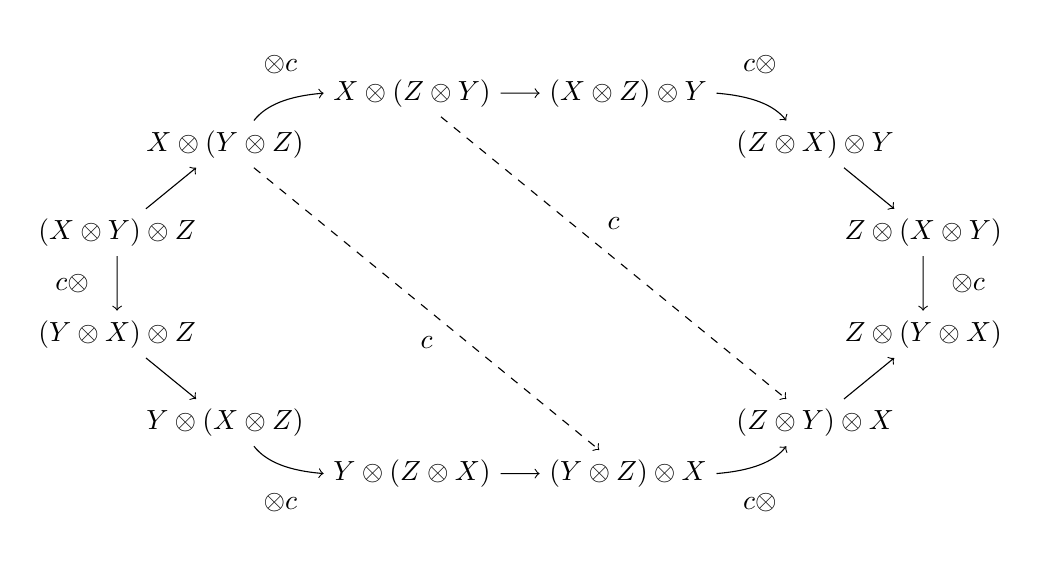
\begin{tikzpicture}[xscale=5.3, yscale=2.5, every edge/.style={draw, ->}, C/.style={inner sep=1em}]
		\node (A1) at (75:1cm) {$(X \otimes Z) \otimes Y$};
		\node (A2) at (105:1cm) {$X \otimes (Z \otimes Y)$};
		\node (A3) at (135:1cm) {$X \otimes (Y \otimes Z)$};
		\node (A4) at (165:1cm) {$(X \otimes Y) \otimes Z$};
		\node (A5) at (195:1cm) {$(Y \otimes X) \otimes Z$};
		\node (A6) at (225:1cm) {$Y \otimes (X \otimes Z)$};
		\node (A7) at (255:1cm) {$Y \otimes (Z \otimes X)$};
		\node (A8) at (285:1cm) {$(Y \otimes Z) \otimes X$};
		\node (A9) at (315:1cm) {$(Z \otimes Y) \otimes X$};
		\node (A10) at (345:1cm) {$Z \otimes (Y \otimes X)$};
		\node (A11) at (15:1cm) {$Z \otimes (X \otimes Y)$};
		\node (A12) at (45:1cm) {$(Z \otimes X) \otimes Y$};

		\draw (A4) edge (A3);	\draw (A3) edge[bend left] node[C, above] {$\identity \otimes c$} (A2); \draw (A2) edge (A1); \draw (A1) edge[bend left] node[C, above] {$c \otimes \identity$} (A12); \draw (A12) edge (A11); \draw (A11) edge node[C, right] {$\identity \otimes c$} (A10);

		\draw (A4) edge node[C, left] {$c \otimes \identity$} (A5); \draw (A5) edge (A6); \draw (A6) edge[bend right] node[C, below] {$\identity \otimes c$} (A7); \draw (A7) edge (A8); \draw (A8) edge[bend right] node[C, below] {$c \otimes \identity$} (A9); \draw (A9) edge (A10);
	
		\draw[dashed] (A3) edge node[C, below] {$c$} (A8);
		\draw[dashed] (A2) edge node[C, above] {$c$} (A9);
	\end{tikzpicture}\end{center}
	Di sini semua panah tanpa label adalah kendala asosiativitas, sedangkan $c$ menyatakan kendala komutativitas yang jelas dari konteks.
\end{proposition}
\begin{proof}
	Garis-garis putus-putus membagi diagram besar menjadi tiga bagian. Bagian kiri dan kanan komutatif karena aksioma segienam. Segi empat di tengah komutatif karena naturalitas $c$. Jadi, seluruh diagram komutatif.
\end{proof}

\begin{remark}\label{rem:YBE-cat-strict}
	Jika $\mathcal{V}$ kategori monoidal ketat, diagram di atas menyusut menjadi enam suku dan komutativitasnya tidak lain menyatakan
	\begin{multline*}
		(c(Y,Z) \otimes \identity_X) \, (\identity_Y \otimes c(X, Z)) \, (c(X, Y) \otimes \identity_Z) = \\
		(\identity_Z \otimes c(X, Y)) \, (c(X, Z) \otimes \identity_Y) \, (\identity_X \otimes c(Y, Z)).
	\end{multline*}
	Jika $\mathcal{V}$ adalah kategori ruang vektor yang membentuk kategori monoidal berkepang terhadap hasil kali tensor dan $X=Y=Z$, kesamaan di atas berkaitan dengan persamaan Yang--Baxter dalam fisika statistik (``Yang'' merujuk kepada Chen-Ning Yang). Penjelasan lebih lanjut akan diberikan dalam latihan.
\end{remark}

\begin{example}\label{eg:braid}\index[sym1]{Braid@$\cate{Braid}$}
	Berikut ini kita membangun kategori kepang \cate{Braid} dari sudut pandang topologis. Misalkan $n \in \Z_{\geq 1}$ dan definisikan
	\[ C_n := \left\{ \text{subhimpunan}\; c \subset \R^2: |c|=n \right\}, \]
	atau, dengan kata lain, ruang hasil bagi $\left\{ (y_1, \ldots, y_n) \in (\R^2)^n: \text{unsur-unsurnya berbeda} \right\}$ oleh aksi grup permutasi; ruang ini secara natural dilengkapi suatu topologi. Mulai sekarang, tetapkan $p = \{p_1, \ldots, p_n\} \in C_n$. Sebuah kepang dengan $n$ untai didefinisikan sebagai peta kontinu $x: [0,1] \to C_n$ yang memenuhi $x(0) = x(1) = p$. Secara visual, jika waktu $t$ dijadikan sumbu vertikal, lintasan $x$ memberikan $n$ kurva kontinu dalam $\R^3$ yang masing-masing tidak berpotongan dengan dirinya sendiri dan saling tidak berpotongan, serta bergerak naik dari $\{(p_1, 0), \ldots, (p_n, 0) \}$ ke $\{ (p_1, 1), \ldots, (p_n, 1) \}$; inilah yang disebut kepang. Jika kepang $x_1$ dapat dideformasi secara kontinu menjadi $x_2$ dengan titik-titik ujung $p$ tetap sepanjang deformasi, maka $x_1$ dan $x_2$ disebut ekuivalen. Selanjutnya, istilah kepang selalu berarti kelas ekuivalensi. Himpunan semua kepang dengan $n$ untai dinotasikan dengan $\mathcal{B}_n$.

	Meskipun kepang dapat dipandang sebagai gambar dalam $\R^3$, kita lazim meratakannya pada suatu bidang $L \simeq \R^2$. Proses ini dapat membuat proyeksi kurva-kurva tersebut berpotongan, tetapi dengan perturbasi kecil pada $L$ dapat dipastikan bahwa proyeksi tiga kurva tidak pernah bertemu pada satu titik. Tanpa mengurangi keumuman, dapat pula diasumsikan bahwa ujung-ujung bawah dan atas kepang masing-masing dipetakan ke $(i, 0), (i, 1) \in \R^2$, dengan $i=1, \ldots, n$. Untuk mempertahankan informasi ruangnya, pada setiap titik potong proyeksi dua kurva kita tandai kurva mana yang melintas di atas dan mana yang di bawah. Sebagai contoh, perhatikan kasus $n=3$:
	\begin{center}\begin{tikzpicture}[baseline=(braid), yscale=0.75]
		\braid[style strands={1}, style strands={2}, style strands={3}] (braid) s_1 s_2^{-1};
		\node[left=1em] (A) at (braid-1-s) {$t=1$};
		\node[left=1em] (B) at (braid-2-e) {$t=0$};
		\draw[-Latex, ultra thick] (B) -- (A);
		\node[below] at (braid-1-e) {$3$};
		\node[below] at (braid-2-e) {$1$};
		\node[below] at (braid-3-e) {$2$};
	\end{tikzpicture} \quad dan \quad \begin{tikzpicture}[baseline=(braid), yscale=0.75]
		\braid[style strands={1}, style strands={2}, style strands={3}] (braid)  s_2 s_1^{-1};
		\node[below] at (braid-1-e) {$2$};
		\node[below] at (braid-2-e) {$3$};
		\node[below] at (braid-3-e) {$1$};
	\end{tikzpicture}\end{center}

	Untuk sebarang $x, y \in \mathcal{B}_n$, definisikan komposisi $xy$ dengan menyambungkan peta $x,y: [0,1] \to C_n$ dari ujung ke ujung; secara visual, ini berarti merekatkan ujung awal $x$ pada ujung akhir $y$ untuk memperoleh kepang baru. Mudah dilihat bahwa operasi ini terdefinisi dengan baik. Sebagai contoh, jika kedua kepang di atas berturut-turut dinotasikan dengan $x,y$, maka
	\[ xy \; = \;
		\begin{array}{|c|c|} \hline x \\ \hline y \\ \hline \end{array} \quad = \quad
		\begin{tikzpicture}[yscale=0.75, baseline=(braid)]
		\braid[style strands={1}, style strands={2}, style strands={3},
			floor command={
			\draw[dashed] (\floorsx,\floorsy) -- (\floorex,\floorsy);
			}] (braid)
		s_1 s_2^{-1} | s_2 s_1^{-1};
	\end{tikzpicture}\]
	Dengan meluruskan setiap untai pada gambar di atas, terlihat bahwa kepang tersebut ekuivalen dengan tiga untai vertikal $\vert\;\vert\;\vert$. Dari sudut pandang aljabar, $\mathcal{B}_n$ bersama operasi komposisi kepang membentuk grup yang disebut \emph{grup kepang Artin}. Asosiativitas perkalian sudah jelas, sedangkan unsur satuannya adalah $\underbracket{\vert \cdots \vert}_{n \text{untai}}$, atau, dengan kata lain, fungsi konstan $[0,1] \to \{p\} \subset C_n$. Invers suatu kepang $x$ diperoleh dengan menelusuri kurva $x: [0,1] \to C_n$ dalam arah sebaliknya, atau, setelah diratakan pada bidang $\R^2$, dengan mengambil cerminan vertikalnya. Pembaca yang mengenal topologi akan segera melihat bahwa $\mathcal{B}_n = \pi_1(C_n, p)$; lihat Contoh \ref{eg:fundamental-groupoid}.

	Dengan konvensi, $\mathcal{B}_0$ adalah grup trivial. Dalam \S\ref{sec:symmetric-group}, kita akan menyelidiki beberapa sifat $\mathcal{B}_n$ dari sudut pandang teori grup serta hubungannya dengan grup simetris $\mathfrak{S}_n$; suatu presentasi grup $\mathcal{B}_n$ akan diberikan dalam \eqref{eqn:braid-presentation}.\index{bianqun@grup kepang (braid group)}\index[sym1]{B_n@$\mathcal{B}_n$}

	Sekarang kita bangun kategori monoidal ketat $\cate{Braid}$: himpunan objeknya adalah $\Z_{\geq 0}$, sedangkan himpunan morfisme antara sebarang dua objek $n,m$ didefinisikan sebagai $\mathcal{B}_n$ jika $n=m$, dan sebagai himpunan kosong jika tidak. Komposisi morfisme adalah komposisi dalam grup kepang. Selanjutnya, definisikan $m \otimes n := m+n$; untuk $x \in \mathcal{B}_m$, $y \in \mathcal{B}_n$, morfisme $x \otimes y \in \mathcal{B}_{m+n}$ didefinisikan dengan menempatkan kedua kepang berdampingan, yang secara visual dinyatakan sebagai
	\begin{center} 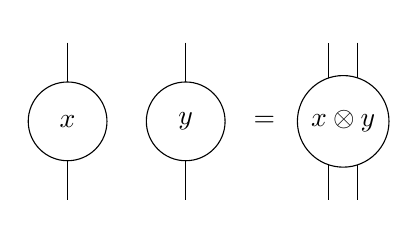
\begin{tikzpicture}[baseline=(current bounding box.center),
		 midbraid/.style={midway, draw, fill=white, shape=circle, minimum size=1cm} ]
		\draw (0,1) -- (0,-1) node[midbraid] {$x$};
		\draw (1.5,1) -- (1.5,-1) node[midbraid] {$y$};
		\node at (2.5,0) {$=$};
		\draw[double distance=10pt] (3.5, 1) -- (3.5,-1) node[midbraid] {$x \otimes y$};
	\end{tikzpicture}\end{center}
	Jelas bahwa $x \otimes y$ terdefinisi dengan baik, dan operasi ini menjadikan $\cate{Braid}$ kategori monoidal ketat; objek satuannya adalah $0$.

	Sekarang definisikan kendala komutativitas $c$ untuk memperoleh kategori monoidal berkepang. Untuk $X=m$, $Y=n$, kita menggunakan
	
\begin{tikzpicture} \draw[black, line width=3pt] (0,0) -- (0.5, 0); \end{tikzpicture}
	untuk menyatakan $m$ untai tak terjalin yang bersesuaian dengan objek $X$, sedangkan
	
\begin{tikzpicture} \draw[lightgray, line width=3pt] (0,0) -- (0.5, 0); \end{tikzpicture}
	menyatakan $n$ untai tak terjalin yang bersesuaian dengan objek $Y$. Definisikan $c(X, Y) \in \mathcal{B}_{m+n}$ sebagai
	\[ c(m,n) \;= \; \begin{tikzpicture}[baseline=(braid)]
		\braid[style strands={1}{lightgray}, style strands={2}{black}, line width=3pt] (braid) s_1;
		\node[above] at (braid-1-s) {$n$};
		\node[above] at (braid-2-s) {$m$};
		\node[below] at (braid-1-e) {$n$};
		\node[below] at (braid-2-e) {$m$};
	\end{tikzpicture}\]
	Ini berarti bahwa $n$ untai 
\begin{tikzpicture} \draw[lightgray, line width=3pt] (0,0)--(0.5,0); \end{tikzpicture} dipandang sebagai satu kesatuan dan dilintaskan di atas $m$ untai yang dinyatakan oleh 
\begin{tikzpicture} \draw[black, line width=3pt] (0,0)--(0.5,0); \end{tikzpicture}. Jika $X$ atau $Y$ selanjutnya dibagi menjadi dua kelompok $U, V$ dan diagram kepang yang bersesuaian digambar (berbentuk
	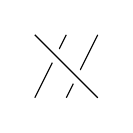
\begin{tikzpicture}[baseline=(current bounding box.center), scale=0.4, wline/.style={color=white, line width=1.8mm}]
		\draw (1,2) -- (0,0);
		\draw (2,2) -- (1,0);
		\draw[wline] (0,2) -- (2,0); \draw (0,2) -- (2,0);
	\end{tikzpicture}
	atau
	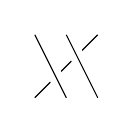
\begin{tikzpicture}[baseline=(current bounding box.center), scale=0.4, wline/.style={color=white, line width=1.8mm}]
		\draw (2,2) -- (0,0);
		\draw[wline] (0,2) -- (1,0); \draw (0,2) -- (1,0);
		\draw[wline] (1,2) -- (2,0); \draw (1,2) -- (2,0);
	\end{tikzpicture} ),
	aksioma segienam dapat diverifikasi (Catatan \ref{rem:hexagon-axiom-strict}); perinciannya diserahkan kepada pembaca.

	Persamaan Yang--Baxter (Catatan \ref{rem:YBE-cat-strict}) dapat diterjemahkan menjadi kesamaan yang langsung terlihat:
	\[ \begin{tikzpicture}[yscale=0.6, baseline=(braid)]
		\braid[style strands={1}, style strands={2}, style strands={3}] (braid) s_1 s_2 s_1;
	\end{tikzpicture}
	\qquad = \qquad
	\begin{tikzpicture}[yscale=0.6, baseline=(braid)]
		\braid[style strands={1}, style strands={2}, style strands={3}] (braid) s_2 s_1 s_2;
	\end{tikzpicture} \]

	Dengan cara yang sama, naturalitas kendala komutativitas dapat ditafsirkan secara intuitif sebagai berikut.
	\begin{center}
	$\begin{tikzcd}
		X \otimes Y \arrow[d, "{f \otimes g}"'] \arrow[r, "{c(X, Y)}"] & Y \otimes X \arrow[d, "{g \otimes f}"] \\
		X' \otimes Y' \arrow[r, "{c(X', Y')}"'] & Y' \otimes X'
	\end{tikzcd}$ \quad komutatif ekuivalen dengan \quad
	\begin{tikzpicture}[baseline=(braid),
		midbraid/.style={shape=circle, draw, fill=white, thick, outer sep=0pt, inner sep=0pt, minimum size=5mm} ]
		\coordinate (B1) at (0, 0);
		\coordinate (B2) at (2.2, 0);
		\braid[style strands={1}{lightgray}, style strands={2}{black}, line width=3pt] (bone) at (B1) s_1;
		\node at (bone-1-s) [midbraid, below=3pt] {\small $g$};
		\node at (bone-2-s) [midbraid, below=3pt] {\small $f$};
		\braid[style strands={1}{lightgray}, style strands={2}{black}, line width=3pt] (btwo) at (B2) s_1;
		\node at (btwo-1-e) [midbraid, above=3pt] {\small $g$};
		\node at (btwo-2-e) [midbraid, above=3pt] {\small $f$};
		\node at ($(bone.center)!.5!(btwo.center)$) {$=$};
	\end{tikzpicture}\end{center}
	Karena
	\begin{tikzpicture}[baseline=(braid), scale=0.5]
		\braid[style strands={1}{black}, style strands={2}{black}] (braid) s_1;
	\end{tikzpicture} $\neq$
	\begin{tikzpicture}[baseline=(braid), scale=0.5]
		\braid[style strands={1}{black}, style strands={2}{black}] (braid) s_1^{-1};
	\end{tikzpicture},
	kategori monoidal $\cate{Braid}$ tidak simetris; sesungguhnya, $c(1, 1)$ membangkitkan grup siklik tak hingga $\mathcal{B}_2 \simeq \Z$, sebagaimana tampak secara intuitif.
\end{example}

Kita telah mengandalkan intuisi topologis untuk memverifikasi semua sifat struktur kepang pada $\cate{Braid}$. Sebaliknya, dapat dibuktikan bahwa segala relasi yang dipenuhi morfisme-morfisme dalam $\cate{Braid}$ terhadap komposisi, yakni berbagai kesamaan diagram kepang, sudah mencakup semua sifat umum kategori monoidal berkepang \cite[Corollary 2.6]{JS93}; dalam ``jargon'' matematikawan, $\cate{Braid}$ adalah ``kategori monoidal berkepang bebas yang dibangkitkan oleh objek $1$''. Dengan kata lain, sifat umum kategori monoidal berkepang dapat diperiksa secara intuitif dalam $\cate{Braid}$. Dibandingkan dengan aksioma-aksioma pada Definisi \ref{def:braiding}, kesamaan antardiagram kepang sering kali langsung terlihat; pembaca kiranya telah menyaksikannya dengan jelas dalam pembahasan persamaan Yang--Baxter.

\section{Kategori Diperkaya}\label{sec:enriched-cat}
Sebenarnya, kita telah menjumpai cukup banyak kategori diperkaya. Kategori diperkaya dapat dipandang dari dua sudut:
\begin{compactitem}
	\item kategori diperkaya merupakan suatu perluasan teori kategori;
	\item kategori diperkaya adalah kategori yang himpunan $\Hom$-nya dilengkapi struktur tambahan.
\end{compactitem}
Sudut pandang pertama memudahkan pengembangan teori dan akan kita gunakan, sedangkan matematikawan biasanya lebih condong pada sudut pandang kedua. Dalam Contoh \ref{eg:categories}, kita telah melihat banyak contohnya; himpunan $\Hom$ dalam kategori-kategori tersebut sering membawa berbagai struktur tambahan, seperti grup abelian atau ruang topologis. Gagasan teori kategori diperkaya ialah
\begin{center}\begin{tikzpicture}
	\node (A) at (0,0) {himpunan-$\Hom$};
	\node (B) at (4,0) {objek-$\Hom$};
	\node[single arrow, draw] at ($(A)!.5!(B)$) {\footnotesize diganti dengan};
\end{tikzpicture}\end{center}
Namun, objek yang disebut terakhir itu merupakan objek dalam kategori apa? Kita harus dapat mendefinisikan komposisi di antara objek-$\Hom$ serta morfisme identitas di dalamnya; kategori monoidal menyediakan bahasa yang sesuai untuk tujuan ini. Monograf mengenai kategori diperkaya dapat dilihat dalam \cite{Ke05}.

\begin{definition}\label{def:enriched-cat}\index{chongshifanchou@kategori diperkaya (enriched category)}
	Misalkan $\mathcal{V}$ kategori monoidal. Yang dimaksud dengan kategori yang diperkaya atas $\mathcal{V}$, atau kategori-$\mathcal{V}$ $\mathcal{C}$, ialah data berikut: \index[sym1]{HomCi@$\iHom_{\mathcal{C}}(X, Y)$}
	\begin{enumerate}
		\item himpunan objek $\Obj(\mathcal{C})$;
		\item untuk setiap dua objek $X, Y \in \Obj(\mathcal{C})$, diberikan objek morfisme $\iHom_{\mathcal{C}}(X, Y) \in \Obj(\mathcal{V})$;
		\item untuk setiap tiga objek $X, Y, Z \in \Obj(\mathcal{C})$, diberikan morfisme komposisi
			\[ M: \iHom_{\mathcal{C}}(Y, Z) \otimes \iHom_{\mathcal{C}}(X, Y) \longrightarrow \iHom_{\mathcal{C}}(X, Z), \]
			seperti biasa, kita akan sering menghilangkan simbol $M$ dan menulis $\iHom_{\mathcal{C}}(\cdots)$ sebagai $\iHom(\cdots)$;
		\item untuk setiap objek $X \in \Obj(\mathcal{C})$, diberikan morfisme identitas
			\[ \identity_X : \munit \to \iHom_{\mathcal{C}}(X ,X); \]
	\end{enumerate}
	sedemikian sehingga diagram-diagram berikut komutatif untuk setiap $X, Y, Z, W \in \Obj(\mathcal{C})$.
	\begin{center} 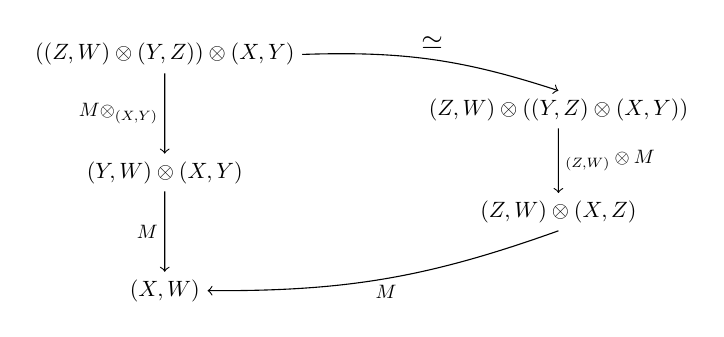
\begin{tikzpicture}[A/.style={scale=0.8, transform shape}, B/.style={scale=0.7, transform shape}, every edge/.style={->, draw}]
		\node[A] (A1) at (0, 3) {$(\iHom(Z, W) \otimes \iHom(Y, Z)) \otimes \iHom(X,Y)$};
		\node[A] (A2) at (0, 1.5) {$\iHom(Y,W) \otimes \iHom(X,Y)$};
		\node[A] (A3) at (0, 0) {$\iHom(X, W)$};
		\node[A] (A4) at (5, 1) {$\iHom(Z,W) \otimes \iHom(X, Z)$};
		\node[A] (A5) at (5, 2.3) {$\iHom(Z,W) \otimes (\iHom(Y,Z) \otimes \iHom(X,Y))$};

		\draw (A1) edge node[B, left] {$M \otimes \identity_{\iHom(X,Y)}$} (A2);
		\draw (A2) edge node[B, left] {$M$} (A3);
		\draw (A4.south) edge[bend left=10] node[B, below] {$M$} (A3.east);
		\draw (A5) edge node[B, right] {$\identity_{\iHom(Z, W)} \otimes M$} (A4);
		\draw (A1.east) edge[bend left=10] node[above]{$\simeq$} (A5.north);
	\end{tikzpicture} \\ \vspace{1.5em}
	\begin{tikzpicture}[A/.style={scale=0.8, transform shape}, B/.style={auto, scale=0.65, transform shape}, every edge/.style={->, draw}]
		\node[A] (T1) {$\iHom(Y, Y) \otimes \iHom(X,Y)$};
		\node[A] (T2) [below=of T1] {$\iHom(X,Y)$};
		\node[A] (T3) [left=of T2] {$\munit \otimes \iHom(X, Y)$};
		\draw (T3.north) edge node[B] {$\identity_Y \otimes \identity_{\iHom(X,Y)}$} (T1.west);
		\draw (T1) edge node[B] {$M$} (T2);
		\draw (T3) edge (T2);
		
		\node[A] (S1) [right=of T1] {$\iHom(X, Y) \otimes \iHom(X,X)$};
		\node[A] (S2) [below=of S1] {$\iHom_{\mathcal{C}}(X,Y)$};
		\node[A] (S3) [right=of S2] {$\iHom(X, Y) \otimes \munit$};
		\draw (S3.north) edge node[B, swap] {$\identity_{\iHom(X,Y)} \otimes \identity_X$} (S1.east);
		\draw (S1) edge node[B, swap] {$M$} (S2);
		\draw (S3) edge (S2);
	\end{tikzpicture} \end{center}
\end{definition}

Jelas bahwa diagram-diagram komutatif di atas hanyalah versi dalam kategori monoidal dari sifat-sifat morfisme pada Definisi \ref{def:category}. Selanjutnya kita bahas fungtor antarkategori-$\mathcal{V}$. Pembaca mungkin sudah dapat menduganya, tetapi tetap kami uraikan secara lengkap.

\begin{definition}\label{def:enriched-functor}\index{hanzi@fungtor!kasus diperkaya}
	Untuk kategori-$\mathcal{V}$ $\mathcal{C}_1$ dan $\mathcal{C}_2$ yang diberikan, suatu fungtor $F: \mathcal{C}_1 \to \mathcal{C}_2$ ditentukan oleh peta di antara himpunan objek $X \mapsto FX$ dan morfisme antarobjek-$\Hom$, yaitu $\iHom(X, Y) \to \iHom(FX, FY)$, sedemikian sehingga diagram-diagram berikut komutatif untuk semua objek $X, Y, Z$.
	\[ \begin{tikzcd}
		\iHom(Y, Z) \otimes \iHom(X, Y) \arrow[r] \arrow[d] & \iHom(X, Z) \arrow[d] \\
		\iHom(FY, FZ) \otimes \iHom(FX, FY) \arrow[r] & \iHom(FX, FZ)
	\end{tikzcd} \]
	\[ \begin{tikzcd}
		\iHom(X, X) \arrow[rr] & & \iHom(FX, FX) \\
		& \munit \arrow[lu] \arrow[ru] &
	\end{tikzcd} \]
\end{definition}

\begin{remark}\label{rem:enriched-to-ordinary}
	Untuk kategori-$\mathcal{V}$ $\mathcal{C}$, dapat didefinisikan kategori biasa yang bersesuaian sebagai berikut: himpunan objeknya tetap $\Obj(\mathcal{C})$, sedangkan himpunan morfismenya ditetapkan sebagai
	\[ \Hom(X, Y) := \Hom_{\mathcal{V}}\left( \munit, \iHom(X, Y) \right). \]
	Dengan demikian, morfisme identitas $\identity_X: \munit \to \iHom(X, X)$ merupakan unsur $\Hom(X, X)$, dan komposisi morfisme didefinisikan melalui
	\[ \begin{tikzcd}
		\Hom_{\mathcal{V}}\left( \munit, \iHom(Y, Z) \right) \times \Hom_{\mathcal{V}}\left( \munit, \iHom(X, Y) \right) \arrow[d, "{\text{fungtorialitas }\;\otimes}"] \\
		\Hom_{\mathcal{V}}\left( \munit \otimes \munit, \iHom(Y, Z) \otimes \iHom(X, Y) \right) \arrow[d, "{\text{tarik balik melalui }\; \iota: \munit \otimes \munit \rightiso \munit \text{ di atas}}"] \\
		\Hom_{\mathcal{V}}\left( \munit, \iHom(X, Z) \right).
	\end{tikzcd} \]
\end{remark}

\begin{definition}\label{def:enriched-naturaltrans}\index{ziranbianhuan@transformasi natural!kasus diperkaya}
	Misalkan $F, G: \mathcal{C}_1 \to \mathcal{C}_2$ fungtor antarkategori-$\mathcal{V}$. Suatu transformasi natural (atau morfisme) $\theta: F \to G$ ialah keluarga morfisme $\theta_X: \munit \to \iHom(FX, GX)$, dengan $X$ merentang seluruh $\Obj(\mathcal{C}_1)$, sedemikian sehingga diagram berikut komutatif untuk semua $X, Y$.
	\[ \begin{tikzcd}
		\munit \otimes \iHom(X, Y) \arrow[r, "{\theta_Y \otimes F}"] & \iHom(FY, GY) \otimes \iHom(FX, FY) \arrow[d] \\
		\iHom(X, Y) \arrow[u] \arrow[d] & \iHom(FX, GY) \\
		\iHom(X, Y) \otimes \munit \arrow[r, "{G \otimes \theta_X}"'] & \iHom(GX, GY) \otimes \iHom(FX, GX) \arrow[u] .
	\end{tikzcd} \]
\end{definition}
Definisi ini tampak berbelit karena, dalam kategori-$\mathcal{V}$ umum, kita tidak dapat membicarakan unsur-unsur objek-$\Hom$. Definisi komposisi vertikal dan horizontal transformasi natural diserahkan kepada pembaca. Versi diperkaya dari fungtor dan transformasi natural memungkinkan kita mendefinisikan gagasan ekuivalensi kategori bagi kategori-$\mathcal{V}$.\index{fanchoudengjia@ekuivalensi kategori!kasus diperkaya}

\begin{example}
	Ambil $\mathcal{V} = \cate{Set}$ dengan $\otimes := \times$ sehingga menjadi kategori monoidal (Contoh \ref{eg:monoidal-cat}); maka kategori-$\mathcal{V}$ tidak lain adalah kategori yang telah didefinisikan sebelumnya. Perhatikan bahwa kita tetap mengikuti Konvensi \ref{con:U-small}, sehingga $\cate{Set}$ adalah kategori yang terdiri atas himpunan-$\mathcal{U}$ dan kategori berarti kategori-$\mathcal{U}$.
\end{example}

\begin{example}\index{tuopufanchou@kategori topologis (topological category)}
	Serupa dengan itu, ambil $\mathcal{V} = \cate{CGHaus}$ (Contoh \ref{eg:categories}) dan $\otimes := \times$. Kategori diperkaya yang bersesuaian disebut \emph{kategori topologis}. Alasan penggunaan $\cate{CGHaus}$ dapat dilihat dalam pembahasan pada Contoh \ref{eg:categories}, atau dalam \cite[Chapter 5]{May99}. 
\end{example}

\begin{example}\label{eg:Ab-cat}\index{Ab-fanchou@kategori-$\cate{Ab}$}
	Ambil $\mathcal{V} := \cate{Ab}$, dengan $\otimes$ hasil kali tensor grup abelian (yakni modul-$\Z$) dan $\munit := \Z$. Kategori-$\cate{Ab}$ yang diperoleh juga disebut \emph{kategori praaditif}. Sebenarnya, kategori-$\cate{Ab}$ dapat didefinisikan tanpa bahasa kategori monoidal. Pada intinya, ciri-ciri kategori-$\cate{Ab}$ adalah sebagai berikut.
	\begin{compactitem}
		\item Setiap himpunan $\Hom$ dilengkapi struktur grup abelian.
		\item Peta komposisi $\Hom(Y, Z) \times \Hom(X, Y) \to \Hom(X, Z)$ adalah peta $\Z$-bilinear, yakni memenuhi $f(g+h) = fg+ fh$ dan $(g+h)f = gf + hf$. Hal ini karena, menurut sifat hasil kali tensor, homomorfisme grup $\Hom(Y,Z) \dotimes{\Z} \Hom(X, Y) \to \Hom(X, Z)$ sama artinya dengan peta bilinear $\Hom(Y, Z) \times \Hom(X, Y) \to \Hom(X, Z)$.
		\item Dengan menguraikan definisi, terlihat bahwa fungtor antarkategori-$\cate{Ab}$ adalah fungtor yang menginduksi homomorfisme grup pada himpunan-himpunan $\Hom$.
		\item Tidak ada syarat tambahan pada transformasi natural.
	\end{compactitem}
	 Semua ini sesuai dengan sudut pandang yang disebutkan pada awal bagian ini; verifikasi terperinci diserahkan sebagai latihan. Secara khusus, untuk semua objek $X, Y$, dalam $\Hom(X, Y)$ terdapat unsur nol $0$ yang terdefinisi dengan baik, dan komposisinya dengan setiap morfisme yang dapat dikomposisikan tetap merupakan unsur nol. Kategori semacam ini sangat umum: misalnya, untuk sebarang gelanggang $A$, kategori modul kiri $A\dcate{Mod}$ adalah kategori-$\cate{Ab}$, termasuk $\cate{Ab}$ itu sendiri.

	Dalam contoh $\cate{Ab}$, untuk setiap grup abelian $M$ terdapat bijeksi natural
	\begin{align*}
		\Hom_{\cate{Ab}}(\Z, M) & \rightiso M \\
		f & \mapsto f(1),
	\end{align*}
	maka terlihat bahwa fungtor $\Hom_{\cate{Ab}}(\munit, \cdot) = \Hom_{\cate{Ab}}(\Z, \cdot): \cate{Ab} \to \cate{Set}$ isomorfik dengan fungtor pelupa. Karena itu, menerapkan prosedur pada Catatan \ref{rem:enriched-to-ordinary} kepada kategori-$\cate{Ab}$ hanya melupakan struktur grup pada himpunan-himpunan $\Hom$.
\end{example}

Karena kategori-$\cate{Ab}$ sering digunakan dalam matematika, selanjutnya kita kaji beberapa sifat khususnya. Ingat kembali \S\ref{sec:limits}. Jika $I$ himpunan kecil, telah diketahui bahwa dalam kategori $A\dcate{Mod}$ terdapat, dengan $I$ sebagai himpunan indeks, produk $\prod_{i \in I} M_i$ dan koproduk $\bigoplus_{i \in I} M_i$ (yakni jumlah langsung modul). Jika $I$ berhingga, keduanya sama: hal ini langsung terlihat dari definisi konkret $\prod$ dan $\bigoplus$, tetapi juga merupakan fenomena umum yang dimiliki semua kategori-$\cate{Ab}$. Untuk menjelaskannya, kita perkenalkan gagasan biproduk.

\begin{definition}\label{def:biproduct}\index{shuangji@biproduk (biproduct)}
	Misalkan $\mathcal{C}$ kategori-$\cate{Ab}$ dan $X_1, X_2$ objek di dalamnya. \emph{Biproduk} dari $X_1, X_2$ berarti diagram
	\[ \begin{tikzcd}
		X_1 \arrow[r, yshift=-0.5ex, "\iota_1"'] & Z \arrow[l, yshift=0.5ex, "p_1"'] \arrow[r, yshift=0.5ex, "p_2"] & X_2 \arrow[l, yshift=-0.5ex, "\iota_2"]
	\end{tikzcd} \]
	sedemikian sehingga $p_1 \iota_1 = \identity$, $p_2 \iota_2 = \identity$, dan $\iota_1 p_1 + \iota_2 p_2 = \identity_Z$. Kita juga mengatakan bahwa $Z$ bersama $(\iota_1, \iota_2, p_1, p_2)$ adalah biproduk $X_1$ dan $X_2$. Notasinya ialah $Z = X_1 \oplus X_2$.
\end{definition}
Dengan mengomposisikan persamaan $\iota_1 p_1 + \iota_2 p_2 = \identity_Z$ di kiri oleh $p_2$ dan di kanan oleh $\iota_1$, diperoleh $p_2 \iota_1 = 0$; demikian pula diperoleh $p_1 \iota_2 = 0$. Konstruksi biproduk dapat diiterasikan ke kasus banyak peubah $Z = X_1 \oplus \cdots \oplus X_n$: untuk setiap $1 \leq i \leq n$, diberikan $\begin{tikzcd} X_i \arrow[r, yshift=-0.5ex, "\iota_i"'] & Z \arrow[l, yshift=0.5ex, "p_i"'] \end{tikzcd}$ sedemikian sehingga
\begin{gather*}
	p_i \iota_j = \begin{cases} \identity, & i=j \\ 0, & i \neq j \end{cases} \qquad
	\sum_{i=1}^n \iota_i p_i = \identity_Z.
\end{gather*}

\begin{theorem}\label{prop:biproduct-criterion}
	Misalkan $X_1, X_2$ objek dalam kategori-$\cate{Ab}$ $\mathcal{C}$. Pernyataan-pernyataan berikut ekuivalen:
	\begin{compactenum}[(i)]
		\item produk $X _1\times X_2$ ada;
		\item koproduk $X_1 \sqcup X_2$ ada;
		\item biproduk dari $X_1$ dan $X_2$, yaitu $Z$, ada.
	\end{compactenum}
	Jika salah satu pernyataan tersebut berlaku, maka biproduk $Z$ bersama $(p_1, p_2)$ memberikan produk $X_1$ dan $X_2$, sedangkan $Z$ bersama $(\iota_1, \iota_2)$ memberikan koproduknya.
\end{theorem}
Menurut Lema \ref{prop:product-associativity}, produk dan koproduk berhingga dapat dibangun secara iteratif dari kasus biner. Ini menjelaskan mengapa jumlah langsung berhingga modul sekaligus berperan sebagai produk dan koproduk.
\begin{proof}
	Andaikan biproduk dari $X_1, X_2$, yaitu $Z$, ada. Karena
	\begin{align*}
		p_1 \iota_2 & = p_1 \circ \identity_Z \circ \iota_2 =  p_1 (\iota_1 p_1 + \iota_2 p_2) \iota_2 = (p_1 \iota_1) p_1 \iota_2 + p_1 \iota_2 (p_2 \iota_2)  \\
		& = p_1 \iota_2 + p_1 \iota_2,
	\end{align*}
	maka $p_1 \iota_2 = 0$. Demikian pula, $p_2 \iota_1 = 0$. Untuk morfisme-morfisme yang diberikan $X_1 \xleftarrow{f_1} W \xrightarrow{f_2} X_2$, tetapkan $\phi := \iota_1 f_1 + \iota_2 f_2 : W \to Z$. Dari rumus sebelumnya diperoleh $p_i \phi = f_i$ ($i=1,2$). Sebaliknya, jika $\phi: W \to Z$ memenuhi $p_i \phi = f_i$, maka
	\[ \phi = (\iota_1 p_1 + \iota_2 p_2) \phi = \iota_1 f_1 + \iota_2 f_2 \]
	menentukan $\phi$ secara tunggal. Jadi, $(Z, p_1, p_2)$ memang memenuhi sifat universal produk.

	Sekarang andaikan $X_1 \xleftarrow{p_1} Z \xrightarrow{p_2} X_2$ adalah produk. Untuk $i=1,2$, definisikan $\iota_i: X_i \to Z$ sedemikian sehingga
	\[ \forall j=1,2, \quad  p_j \iota_i =
		\begin{cases}
			\identity_{X_i}, & i=j, \\
			0, & i \neq j .
		\end{cases}
	\]
	Cukup diverifikasi $\iota_1 p_1 + \iota_2 p_2 = \identity_Z$ untuk membuktikan bahwa $(Z, \iota_1, \iota_2, p_1, p_2)$ adalah biproduk. Kita mempunyai
	\begin{align*}
		p_1 (\iota_1 p_1 + \iota_2 p_2) & = p_1 + 0 = p_1 \circ \identity_Z , \\
		p_2 (\iota_1 p_1 + \iota_2 p_2) & = 0 + p_2 = p_2 \circ \identity_Z.
	\end{align*}
	Dari sifat universal produk diperoleh $\iota_1 p_1 + \iota_2 p_2 = \identity_Z$. Kasus koproduk diperoleh dengan membalik arah panah.
\end{proof}
\begin{remark}
	Dengan mencermati pembuktian, terlihat bahwa isomorfisme $\psi: X_1 \sqcup X_2 \rightiso X_1 \times X_2$ dapat dipilih sebagai morfisme yang dicirikan oleh
	\[ p_j \psi \iota_i =
		\begin{cases}
			\identity_{X_i}, & i=j, \\
			0, & i \neq j
		\end{cases} \]
	dengan $\iota_i : X_i \to X_1 \sqcup X_2$ dan $p_i: X_1 \times X_2 \to X_i$.
\end{remark}

\begin{lemma}
	Misalkan $X$ objek dalam kategori-$\cate{Ab}$ $\mathcal{C}$. Sifat-sifat berikut ekuivalen:
	\begin{compactenum}[(i)]
		\item $X$ adalah objek awal,
		\item $\identity_X = 0$,
		\item $\End_{\mathcal{C}}(X) = \{0\}$,
		\item $X$ adalah objek terminal.
	\end{compactenum}
	Secara khusus, jika $X$ objek awal atau objek terminal, maka $X$ adalah objek nol (Definisi \ref{def:universal-objects}), dan $0 \in \Hom(X, \cdot)$ adalah morfisme nol pada Definisi \ref{def:zero-morphism}.
\end{lemma}
\begin{proof}
	Andaikan $X$ objek awal dalam $\mathcal{C}$. Grup $\End_{\mathcal{C}}(X)$ hanya mempunyai satu unsur, yang haruslah $0 = \identity_X$; jadi (i) $\implies$ (ii). Karena untuk setiap $Y$ dan $f \in \Hom(X, Y)$ berlaku $f \circ \identity_X = f$, sifat kategori-$\cate{Ab}$ memberikan (ii) $\implies$ (iii) $\implies$ (i). Dengan membalik arah panah, terlihat bahwa (iv) ekuivalen dengan syarat-syarat lainnya.
\end{proof}

\begin{definition}[Fungtor Aditif dan Kategori Aditif]\label{def:additive-cat}\index{jiaxingfanchou@kategori aditif (additive category)}\index{hanzi@fungtor!kasus aditif}
	Fungtor antarkategori-$\cate{Ab}$ (lihat Definisi \ref{def:enriched-functor}) disebut \emph{fungtor aditif}. Jika kategori-$\cate{Ab}$ $\mathcal{C}$ mempunyai objek nol $0$ dan setiap $X, Y \in \Obj(\mathcal{C})$ mempunyai biproduk $X \oplus Y$, maka $\mathcal{C}$ disebut \emph{kategori aditif}. 
\end{definition}

Kategori modul $A\dcate{Mod}$ yang telah disebutkan sebelumnya adalah contoh khas kategori aditif; lihat Korolari \ref{prop:Mod-cat-additive}. Fungtor $F: \mathcal{C}_1 \to \mathcal{C}_2$ adalah fungtor aditif jika dan hanya jika $\Hom_{\mathcal{C}_1}(X, Y) \to \Hom_{\mathcal{C}_2}(FX, FY)$ merupakan homomorfisme grup aditif untuk setiap $X, Y$.

\begin{proposition}\label{prop:biproduct-preservation}
	Fungtor aditif antarkategori-$\cate{Ab}$ mempertahankan biproduk.
\end{proposition}
\begin{proof}
	Jika $F: \mathcal{C} \to \mathcal{C}'$ fungtor aditif dan data $(\iota_1, \iota_2, p_1, p_2)$ mendefinisikan biproduk dalam $\mathcal{C}$, maka data $(F(\iota_1), F(\iota_2), F(p_1), F(p_2))$ tetap memenuhi syarat-syarat biproduk. Alasannya, biproduk didefinisikan oleh persamaan, bukan oleh keberadaan panah.
\end{proof}

\begin{proposition}\label{prop:additive-prod-coprod}
	Dalam kategori aditif, produk dan koproduk sebarang keluarga berhingga objek ada dan keduanya isomorfik secara natural.
\end{proposition}
\begin{proof}
	Kasus dua objek tidak lain adalah Teorema \ref{prop:biproduct-criterion} tentang biproduk; kasus umum direduksi ke kasus dua objek melalui kendala asosiativitas pada Lema \ref{prop:product-associativity}.
\end{proof}

\section{Sekilas tentang \texorpdfstring{$2$}{2}-Kategori}\label{sec:2-cat}
Kita telah terbiasa menggambarkan objek suatu kategori sebagai titik dan morfismenya sebagai panah di antara titik-titik tersebut; konstruksi berdimensi tertinggi dalam gambaran ini adalah panah satu dimensi, sehingga kategori wajar disebut $1$-kategori. Kategori yang diperoleh dengan melupakan panah tidak lain adalah himpunan: yang tersisa hanya objek berdimensi nol, sehingga himpunan dapat dipandang sebagai $0$-kategori. Ini menimbulkan pertanyaan yang wajar: bagaimana kategori tingkat lebih tinggi didefinisikan? Bagian ini hanya membahas tingkat $2$; dengan kata lain, selain titik dan panah kita akan menambahkan konstruksi berdimensi $2$ tertentu, yang disebut $2$-sel.

$2$-Kategori bukan khayalan tanpa dasar. Sebagai contoh, $\cate{Cat}$ dalam Contoh \ref{eg:Cat} merupakan contoh baku; contoh alami lainnya diperoleh dengan meninjau ruang topologis (titik), peta kontinu di antaranya (panah), dan homotopi antarpeta ($2$-sel). Meskipun gagasannya sederhana, menyarikan definisi yang tepat merupakan persoalan besar. Versi definisi berikut juga disebut $2$-kategori ketat.

\begin{definition}\index{$2$-kategori}
	Suatu $2$-kategori (ketat) $\mathcal{C}$ terdiri atas data berikut:
	\begin{itemize}
		\item himpunan objek, yang juga disebut $0$-morfisme, $\Obj(\mathcal{C}) = \Mor_0(\mathcal{C})$;
		\item himpunan $1$-morfisme, $\Mor_1(\mathcal{C}) = \bigsqcup_{X, Y \in \Mor_0(\mathcal{C})} \Hom(X, Y)$;
		\item himpunan $2$-morfisme, $\Mor_2(\mathcal{C}) = \bigsqcup_{a, b \in \Mor_1(\mathcal{C})} \Hom(a, b)$.
	\end{itemize}
	Biasanya $1$-morfisme ditulis dalam bentuk $f: X \to Y$, sedangkan $2$-morfisme ditulis dalam bentuk $\theta: a \Rightarrow b$. Di dalam $\mathcal{C}$ terdapat operasi-operasi berikut.
	\begin{enumerate}[(i)]
		\item Kita mensyaratkan bahwa objek-objek $\mathcal{C}$ beserta $1$-morfismenya membentuk suatu kategori ($1$-kategori).
		% Komposisi $1$-morfisme $\Hom(Y, Z) \times \Hom(X, Y) \to \Hom(X, Z)$, dengan $X, Y, Z$ objek; di sini komposisi disyaratkan memenuhi hukum asosiatif, dan untuk setiap objek $X$ terdapat unsur identitas $\identity_X$. Dengan kata lain, objek $\mathcal{C}$ beserta $1$-morfismenya disyaratkan membentuk suatu kategori.
		\item $2$-Morfisme mempunyai dua macam komposisi, yaitu vertikal dan horizontal. Pertama-tama tinjau komposisi vertikal: misalkan $X, Y$ objek, $f, g, h: X \to Y$ merupakan $1$-morfisme, serta $\theta: f \Rightarrow g$ dan $\psi: g \Rightarrow h$ merupakan $2$-morfisme. Maka terdapat komposisi vertikal $\psi \circ \theta: f \Rightarrow h$, yang digambarkan sebagai
			\[ \begin{tikzcd}
				X
				\arrow[bend left=60, rr, "f", ""' name=U]
				\arrow[rr, "g"' name=M, "" name=MM]
				\arrow[bend right=60, rr, "" name=D, "h"'] & &
				\arrow[Rightarrow, to path=(U) -- (MM) \tikztonodes, "\theta"] \arrow[Rightarrow, to path=  (M) -- (D) \tikztonodes, "\psi"]  Y
			\end{tikzcd}
			\quad \text{dikomposisikan menjadi} \quad
			\begin{tikzcd}
				X
				\arrow[bend left=50, rr, "f", ""' name=U]
				\arrow[bend right=50, rr, "" name=D, "h"']
				& & \arrow[Rightarrow, to path=(U) -- (D) \tikztonodes, "\psi \circ \theta"] Y .
			\end{tikzcd} \]
		\item Selanjutnya tinjau komposisi horizontal. Misalkan $X, Y ,Z$ objek, \begin{tikzcd} X \arrow[r, bend left=20, "f"] \arrow[r, bend right=20, "g"'] & Y \end{tikzcd}, \begin{tikzcd} Y \arrow[r, bend left=20, "f'"] \arrow[r, bend right=20, "g'"'] & Z \end{tikzcd} merupakan dua pasang $1$-morfisme, sedangkan $\theta: f \Rightarrow g$ dan $\psi: f' \Rightarrow g'$ merupakan $2$-morfisme. Maka terdapat komposisi horizontal $\psi \circ \theta: f'f \Rightarrow g'g$, yang digambarkan sebagai
			\[ \begin{tikzcd}
				X \arrow[bend left=50, r, "f", ""' name=LU] \arrow[bend right=50, r, "" name=LD, "g"'] &
				Y \arrow[bend left=50, r, "f'", ""' name=RU] \arrow[bend right=50, r, "" name=RD, "{g'}"'] &
				\arrow[Rightarrow, to path=(LU) -- (LD) \tikztonodes, "\theta"] \arrow[Rightarrow, to path=(RU) -- (RD) \tikztonodes, "\psi"] Z
			\end{tikzcd}
			\quad \text{dikomposisikan menjadi} \quad
			\begin{tikzcd}
				X
				\arrow[bend left=40]{rr}{f'f}[name=U, below]{}
				\arrow[bend right=40]{rr}[name=D]{}[below]{g'g}
				& & \arrow[Rightarrow, to path=(U) -- (D) \tikztonodes]{}{\psi \circ \theta} Z .
			\end{tikzcd} \]
	\item Diagram berbentuk
		\begin{tikzcd}
			X
			\arrow[bend left=30]{rr}{f}[name=U, below]{}
			\arrow[bend right=30]{rr}[name=D]{}[below]{g}
			& & \arrow[Rightarrow, to path=(U) -- (D) \tikztonodes]{}{\theta} Y
		\end{tikzcd}
		disebut $2$-sel. Kita mensyaratkan agar komposisi horizontal memenuhi hukum asosiatif secara ketat, $\phi \circ (\psi \circ \theta) = (\phi \circ \psi) \circ \theta$, dan agar untuk setiap objek $X$ terdapat identitas horizontal (atau sebaiknya disebut sel identitas horizontal) $\identity_{X, 2}: \identity_X \Rightarrow \identity_X$, sedemikian sehingga $\theta \circ \identity_{X, 2} = \theta$ dan $\identity_{X, 2} \circ \psi = \psi$ setiap kali komposisi horizontal tersebut terdefinisi.
	\item Demikian pula, komposisi vertikal $2$-sel disyaratkan memenuhi hukum asosiatif secara ketat, dan untuk setiap $1$-morfisme $f$ terdapat identitas vertikal $\identity_f: f \Rightarrow f$.
	\item Komposisi horizontal dari identitas-identitas vertikal tetap merupakan identitas vertikal:
		\[ \begin{tikzcd}
		X \arrow[bend left=50, r, "f", ""' name=LU] \arrow[bend right=50, r, "" name=LD, "f"'] &
		Y \arrow[bend left=50, r, "{f'}", ""' name=RU] \arrow[bend right=50, r, "" name=RD, "{f'}"'] &
		\arrow[Rightarrow, to path=(LU) -- (LD) \tikztonodes, "{\identity_f}"] \arrow[Rightarrow, to path=(RU) -- (RD) \tikztonodes, "{\identity_{f'}}"]  Z
	\end{tikzcd}
	\quad \text{komposisi horizontalnya adalah} \quad
	\begin{tikzcd}
		X
		\arrow[bend left=40, rr, "{f'f}", ""' name=U]
		\arrow[bend right=40, rr, "{f'f}"', "" name=D]
		& & \arrow[Rightarrow, to path=(U) -- (D) \tikztonodes, "{\identity_{f'f}}"] Z .
	\end{tikzcd} \]
	\item Komposisi vertikal dan horizontal memenuhi hukum pertukaran: untuk diagram
		\[ \begin{tikzcd}
			X
			\arrow[bend left=60, rr, ""' name=U]
			\arrow[rr, "" name=MM, ""' name=M]
			\arrow[bend right=60, rr, "" name=D] & &
			\arrow[Rightarrow, to path=(U) -- (MM) \tikztonodes, "\theta"] \arrow[Rightarrow, to path=  (M) -- (D) \tikztonodes, "\psi"] Y
			\arrow[bend left=60, rr, ""' name=V]
			\arrow[rr, "" name=NN, ""' name=N]
			\arrow[bend right=60, rr, "" name=E] & &
			\arrow[Rightarrow, to path=(V) -- (NN) \tikztonodes, "\theta'"] \arrow[Rightarrow, to path=  (N) -- (E) \tikztonodes, "\psi'"] Z
		\end{tikzcd} \]
		berlaku
		\[ \left( \psi' \underset{\text{vertikal}}{\circ} \theta'\right) \underset{\text{horizontal}}{\circ} \left( \psi \underset{\text{vertikal}}{\circ} \theta\right) = \left( \psi' \underset{\text{horizontal}}{\circ} \psi \right) \underset{\text{vertikal}}{\circ} \left( \theta' \underset{\text{horizontal}}{\circ} \theta\right).  \]
	\end{enumerate}
\end{definition}

\begin{remark}
	Definisi di atas jelas bertentangan dengan semangat Catatan \ref{rem:strict-or-not}, sebab komposisi morfisme kita syaratkan memenuhi hukum asosiatif dan sifat identitas secara ketat. Untuk $2$-kategori terdapat versi definisi yang lebih longgar sekaligus jauh lebih rumit, misalnya bikategori; untungnya, bikategori juga memenuhi teorema koherensi, yakni setiap bikategori ekuivalen dengan suatu $2$-kategori (bandingkan dengan definisi kategori monoidal dan teorema koherensinya \ref{prop:ML-coherence}). Fenomena koherensi semacam ini tidak lagi berlaku bagi kategori bertingkat lebih dari $2$. Karena keterbatasan ruang, pembahasan kita cukupkan sampai di sini.
\end{remark}

\begin{example}\label{eg:Cat}\index[sym1]{Cat@$\cate{Cat}$}
	Contoh khas $2$-kategori ialah $\cate{Cat}$, yang untuk sementara dapat dibayangkan secara kasar sebagai ``kategori dari kategori-kategori''; bayangan naif semacam itu segera menghadapi kesulitan teori himpunan. Di sini kita harus memilih suatu semesta Grothendieck $\mathcal{U}$ dan, sesuai Konvensi \ref{con:U-small}, membedakan kategori dari kategori kecil. Sekarang $2$-kategori $\cate{Cat}$ dapat didefinisikan sebagai berikut.
	\begin{compactitem}
		\item Objek atau $0$-morfisme: himpunan semua kategori kecil.
		\item $1$-Morfisme: $\Hom(\mathcal{C}_1, \mathcal{C}_2)$ didefinisikan sebagai himpunan fungtor dari $\mathcal{C}_1$ ke $\mathcal{C}_2$.
		\item $2$-Morfisme: $\Hom(\alpha, \beta)$ didefinisikan sebagai himpunan transformasi natural $\theta: \alpha \to \beta$.
		\item Komposisi $1$-morfisme didefinisikan sebagai komposisi fungtor; komposisi vertikal dan horizontal $2$-morfisme masing-masing didefinisikan sebagai komposisi vertikal dan horizontal transformasi natural.
	\end{compactitem}
	Definisi identitas vertikal dan horizontal sudah jelas sehingga tidak perlu diuraikan lagi. Lema \ref{prop:naturaltrans-associativity} memastikan bahwa $\cate{Cat}$ memenuhi aksioma-aksioma $2$-kategori.
\end{example}

Jika pada $\cate{Cat}$ kita melupakan $2$-morfismenya dan hanya meninjau struktur kategori biasa yang dimilikinya, maka $\cate{Cat}$ mempunyai struktur monoidal alami: operasi $\otimes$ diambil sebagai produk kategori $\times$, sedangkan objek satuannya $\munit$ adalah kategori yang hanya mempunyai satu morfisme (ingat Contoh \ref{eg:categories}). Perhatikan bahwa $\times$ dapat dipahami sebagai produk dalam kategori $\cate{Cat}$, sedangkan $\munit$ merupakan objek terminal $\cate{Cat}$; karena itu, konstruksi ini adalah kasus khusus dari Contoh \ref{eg:monoidal-cat}.

\begin{remark}
	Sekarang $2$-kategori dapat dipahami melalui gagasan kategori diperkaya. Misalkan $\mathcal{C}$ suatu $2$-kategori. Untuk setiap objek $X, Y$, definisikan kategori vertikal $\mathcal{V}(X, Y)$ yang objeknya merupakan $1$-morfisme $f: X \to Y$ dan morfismenya merupakan $2$-morfisme $\theta: f \Rightarrow g$; komposisi morfisme diberikan oleh komposisi vertikal $2$-morfisme. Hukum asosiatif vertikal serta sifat identitas vertikal $\identity_f: f \Rightarrow f$ memastikan bahwa $\mathcal{V}(X, Y)$ memang suatu kategori. Selanjutnya kita andaikan bahwa setiap $\mathcal{V}(X, Y)$ merupakan kategori kecil. Untuk $\cate{Cat}$, kategori vertikal $\mathcal{V}(\mathcal{C}_1, \mathcal{C}_2)$ yang bersesuaian tidak lain adalah kategori fungtor $\text{Fct}(\mathcal{C}_1, \mathcal{C}_2)$ yang didefinisikan pada \S\ref{sec:functor-category}.

	Struktur $2$-kategori $\mathcal{C}$ dapat dirumuskan kembali sebagai berikut:
	\begin{compactitem}
		\item himpunan objek $\Obj(\mathcal{C})$;
		\item untuk setiap $X, Y \in \Obj(\mathcal{C})$, diberikan suatu kategori $\mathcal{V}(X, Y)$;
		\item untuk setiap $X, Y, Z \in \Obj(\mathcal{C})$, diberikan fungtor biner
			\[ \circ: \mathcal{V}(Y, Z) \times \mathcal{V}(X, Y) \to \mathcal{V}(X, Z); \]
		\item untuk setiap $X \in \Obj(\mathcal{C})$, diberikan fungtor
			\[ U_X: \munit \to \mathcal{V}(X, X); \]
		\item kita mensyaratkan agar fungtor $\circ$ memenuhi hukum asosiatif secara ketat dan agar $U_X$ mempunyai sifat unsur identitas terhadap $\circ$.
	\end{compactitem}
	Sesungguhnya, pada tataran objeknya, fungtor $\circ: \mathcal{V}(Y, Z) \times \mathcal{V}(X, Y) \to \mathcal{V}(X, Z)$ memuat operasi komposisi $1$-morfisme; pada tataran morfismenya, fungtor tersebut memuat operasi komposisi horizontal $2$-morfisme. Dapat diperiksa bahwa fungtor itu sekaligus memuat sifat identitas horizontal dan hukum pertukaran dalam definisi $2$-kategori. Memilih fungtor $U_X: \munit \to \mathcal{V}(X, X)$ setara dengan menandai suatu objek dalam $\Hom(X, X)$, dan objek itu tidak lain adalah $\identity_X$.

	Ringkasnya, $2$-kategori tidak lain adalah kategori yang diperkaya atas $\cate{Cat}$: untuk setiap objek $X, Y \in \Obj(\mathcal{C})$, himpunan-$\Hom$ $\Hom(X, Y)$ kita perkaya menjadi kategori vertikal $\iHom(X, Y) := \mathcal{V}(X, Y)$, yang merupakan objek kategori monoidal $\cate{Cat}$. Dengan demikian, kita sampai pada Definisi \ref{def:enriched-cat} tentang kategori diperkaya.
\end{remark}

\begin{definition}
	$2$-Fungtor dan $2$-transformasi natural di antara $2$-kategori didefinisikan menurut konstruksi kategori yang diperkaya atas $\cate{Cat}$ (lihat Definisi \ref{def:enriched-functor}, \ref{def:enriched-naturaltrans}).
\end{definition}
Pembaca dipersilakan mencoba menguraikan definisi-definisi tersebut. Sebagai contoh, definisi $2$-fungtor memetakan $i$-morfisme ke $i$-morfisme (di sini $i=0,1,2$) dan mempertahankan sumber/target, komposisi, identitas, serta sifat-sifat lain dari morfisme tersebut.

\begin{convention}
	Untuk $2$-kategori, kita tetap menggunakan beberapa diagram yang diperkenalkan ketika membahas transformasi natural (yakni $2$-kategori $\cate{Cat}$), misalnya diagram dalam \S\ref{sec:functors} yang berbentuk
	\[ \begin{tikzcd}
		X \arrow[r, "h"] & Y \arrow[bend left=50, r, "f", ""' name=U] \arrow[bend right=50, r, "" name=D, "g"'] & Z \arrow[Rightarrow, to path=(U)--(D) \tikztonodes, "\theta"] \arrow[r, "k"] & W
	\end{tikzcd} \]
	yang komposisi horizontalnya bermakna bahwa masing-masing $1$-morfisme $h, k$ ``dilebarkan'' menjadi $2$-sel $\identity_h, \identity_k$, lalu komposisi horizontal dilakukan. Demikian pula, diagram yang diperkenalkan dalam Catatan \ref{rem:triangle-identity},
	\[\begin{tikzcd}
		{} & X \arrow[rr, "\identity", ""' name=I] \arrow[rd, "f"] \arrow[Rightarrow, d, "\varepsilon"] & & X \\
		Y \arrow[ru, "g"] \arrow[rr, "" name=J, "\identity"'] & {} & Y \arrow[ru, "g"'] \arrow[Leftarrow, to path= -- (I) \tikztonodes, "\eta"] &
	\end{tikzcd} \]
	menyatakan komposisi berikut dalam $2$-kategori:
	\[ \begin{tikzcd}
		Y \arrow[r, "g"] \arrow[bend right=60, rr, "" name=J, "\identity"'] &
		X \arrow[r, "f"] \arrow[bend left=60, rr, "\identity", ""' name=I] \arrow[Rightarrow, to path= --(J) \tikztonodes, "\varepsilon"] &
		Y \arrow[r, "g"] \arrow[Leftarrow, to path= -- (I) \tikztonodes, "\eta"] &
		X .
	\end{tikzcd} \]
\end{convention}

\begin{remark}\index{bansuidui@pasangan adjoin}
	Pasangan adjoin $(F, G, \eta, \varepsilon)$ yang dibahas dalam \S\ref{sec:adjoint-functor} dapat dirumuskan kembali dengan bahasa $2$-kategori. Misalkan
	\[\begin{tikzcd}
		X \arrow[yshift=0.5ex, r, "f"] & Y \arrow[yshift=-0.5ex, l, "g"]
	\end{tikzcd}\]
	di dalam suatu $2$-kategori $\mathcal{C}$ merupakan sepasang $1$-morfisme, sedangkan $\eta: \identity_X \Rightarrow gf$ dan $\varepsilon: fg \Rightarrow \identity_Y$ merupakan $2$-morfisme. Jika keduanya memenuhi identitas segitiga dalam Catatan \ref{rem:triangle-identity}, maka $(f, g, \eta, \varepsilon)$ disebut pasangan adjoin. Dengan mengambil $\mathcal{C} = \cate{Cat}$, kita memperoleh kembali definisi klasik pasangan adjoin. Banyak sifat fungtor adjoin dapat diperluas ke kasus $2$-kategori; misalnya, pembuktian Teorema Ekuivalensi Adjoin \ref{prop:adjoint-equivalence} dapat digunakan tanpa perubahan.
\end{remark}
	
\begin{Exercises}
	\item 对于一般幺半范畴中的对象 $X_1, \ldots, X_{n+1}$, 有种种方式能构作循序的 $n$-重 $\otimes$ 运算, 取决于安插括号的方法, 如 $\cdots \otimes (X_i \otimes X_{i+1}) \cdots$ 等等. 证明括号的放法恰有 $\frac{1}{n+1} \binom{2n}{n}$ 种. \begin{hint} 此即组合学中的 Catalan 数. \end{hint}
	\item 证明对任意幺半范畴, $\End(\munit)$ 对态射的合成交换. \begin{hint} 应用引理 \ref{prop:Kelly} 和 $(f \otimes \identity)(\identity \otimes g) = f \otimes g = (\identity \otimes g) (f \otimes \identity)$.\end{hint}
	\item 考虑全体有限全序集和保序映射所成范畴 $\cate{On}_f$. 对于有限全序集 $\sigma$, $\tau$, 在 $\sigma \sqcup \tau$ 上定义唯一的全序使得 $\sigma$ 和 $\tau$ 到 $\sigma \sqcup \tau$ 的嵌入是保序的, 而且 $\sigma$ 中的元素总小于 $\tau$ 中元素. 证明 $\sqcup$ 赋予 $\cate{On}_f$ 自然的幺半范畴结构, 其幺元是空集.
	\item 承上, 说明存在唯一的同构 $c(\sigma, \tau): \sigma \sqcup \tau \rightiso \tau \sqcup \sigma$, 证明 $(\cate{On}_f, \sqcup, c)$ 构成对称幺半范畴.
	\item 本题假定读者熟悉向量空间的张量积. 令 $V$ 为域 $\Bbbk$ 上的向量空间, $R$ 为 $V \otimes V$ 的线性自同构, 相应的杨--Baxter 方程定义作
		\[ (R \otimes \identity_V) \, (\identity_V \otimes R) \, (R \otimes \identity_V) = (\identity_V \otimes R) \, (R \otimes \identity_V) \, (\identity_V \otimes R) , \]
		其中每一项都是 $V \otimes V \otimes V$ 的线性自同构. 设 $\{e_i\}_{i \in I}$ 是 $V$ 的基, 将 $R$ 按 $R(e_i \otimes e_j) = \sum_{k,l} R^{k,l}_{i,j} e_k \otimes e_l$ 展开, 那么上述方程化作
		\[ \forall i,j,k,l,m,n, \quad \sum_{p,q,y} R^{p,q}_{i,j} R^{y,n}_{q,k} R^{l,m}_{p,y} = \sum_{y,q,r} R^{q,r}_{j,k} R^{l,y}_{i,q} R^{m,n}_{y,r}.  \]
		显然此方程不易求解. 如果 $\mathcal{V}$ 是 $(\cate{Vect}(\Bbbk), \otimes, \ldots)$ 的一个幺半子范畴, 且具有辫结构 $c$, 那么对任意 $V \in \Obj(\mathcal{V})$, 从 $R := c(V,V)$ 可得出杨--Baxter 方程的解. 这些方程和一些量子可积系统密切相关. 这也解释了命题 \ref{prop:YBE-cat-strict} 的背景. 请验证上述论断.
		
		现在引进参数 $q \in \Bbbk^\times$. 对于有限维 $\Bbbk$-向量空间 $V = \bigoplus_{i=1}^h \Bbbk e_i$, 证明
		\[ R(e_i \otimes e_j) = \begin{cases}
			e_j \otimes e_i, & i < j, \\
			q e_i \otimes e_j, & i = j, \\
			e_j \otimes e_i + (q - q^{-1}) e_i \otimes e_j, & i > j
		\end{cases} \]
		给出杨--Baxter 方程的解, 并且满足 $\left( R - q \cdot \identity_{V \otimes V} \right) \left( R + q^{-1} \cdot \identity_{V \otimes V} \right) = 0$. 当 $q=1$ 时它退化为 $\cate{Vect}(\Bbbk)$ 上标准的辫结构 $v \otimes w \mapsto w \otimes v$. \index{YBE}

	\item 设 $(\mathcal{V}, \otimes, \ldots)$ 为幺半范畴. 为简便起见, 以下设其为严格幺半范畴, 省略结合约束等态射和括号. 定义幺半范畴 $Z(\mathcal{V})$ 使得:
		\begin{itemize}
			\item 其对象为 $(X, \Phi)$, 其中 $X$ 是 $\mathcal{V}$ 的对象而 $\Phi: (X \otimes -) \rightiso (- \otimes X)$ 是函子的同构, 我们进一步要求对所有对象 $Y,Z$, 下图交换.
				\[\begin{tikzcd}[column sep=small]
					X \otimes Y \otimes Z \arrow[rr, "\Phi_{Y \otimes Z}"] \arrow[rd, "{\Phi_Y \otimes \identity_Z}"'] & & Y \otimes Z \otimes X \\
					&  Y \otimes X \otimes Z \arrow[ru, "{\identity_Y \otimes \Phi_Z}"'] &
				\end{tikzcd}\]
			\item 从 $(X, \Phi)$ 到 $(Y, \Psi)$ 的态射取为所有满足下式的 $f \in \Hom_{\mathcal{V}}(X,Y)$
				\[ \forall Z \in \Obj(\mathcal{V}),\quad (\identity_Z \otimes f) \Phi_Z = \Psi_Z (f \otimes \identity_Z) \; \in \Hom_{\mathcal{V}}(X \otimes Z, Z \otimes Y); \]
			\item 取 $(X, \Phi) \otimes (Y, \Psi)$ 为 $(X \otimes Y,\; (\Phi \otimes \identity)(\identity \otimes \Psi))$. 定义 $Z(\mathcal{V})$ 之幺元为 $\left(\munit, (\identity_X)_{X \in \Obj(\mathcal{V})}\right)$.
		\end{itemize}
		验证这确实给出幺半范畴. 此外 $Z(\mathcal{V})$ 具有自然的辫结构, 试阐明之. 范畴 $Z(\mathcal{V})$ 称为 $\mathcal{V}$ 的 Drinfeld 中心, 这是幺半群中心的一种范畴化.
	\item 验证例 \ref{eg:Ab-cat} 中 $\cate{Ab}$-范畴的刻画确实符合充实范畴的一般理论.
	\item 对给定的函子 $\mathcal{A} \xrightarrow{S} \mathcal{C} \xleftarrow{T} \mathcal{B}$, 按定义 \ref{def:comma-category} 构造范畴 $(S/T)$ (回忆其对象形如 $(A,B,f)$) 及投影函子 $P,Q$. 定义态射 $\alpha: SP \to TQ$ 为 $SP(A,B,f) = \left[ SA \xrightarrow{f} TB \right] = TQ(A,B,f)$. 证明 $\alpha$ 确实是函子间的态射, 而且
		\[\begin{tikzcd}
			(S/T) \arrow[r, "P"] \arrow[d, "Q"'] & \mathcal{A} \arrow[d, "S"] \arrow[Rightarrow, ld, "\alpha" description] \\
			\mathcal{B} \arrow[r, "T"'] & \mathcal{C}
		\end{tikzcd}\]
		是 $2$-范畴 $\cate{Cat}$ 中的 $2$-胞腔.
\end{Exercises}
